
\chapter{FRONT-END SIGNAL PROCESSING}

\section{Introduction}
\label{sec:intro}
 
Overlapped speech constitutes a significant amount of research in co-channel speech. 
To such an extant that in many cases the terms co-channel and overlapped speech are used interchangeably. 
This chapter focuses on proposing signal processing techniques to recognize instances of co-channel data where speakers overlap; overlapped speech detection. 
Single-channel recordings from meetings or conversations are examples during which speakers may overlap. 
In fact, as shown in the previous chapter, the is a direct relation between the number of speakers and the possibility of overlap. 

Most studies on overlapped speech have focused on separating the target or suppressing interfering speech~\cite{morgan_cochannel}. 
Often to de-noise and thereby improve the performance of automatic speech applications~\cite{Quat_Dan_cch_sup,Chazan_93,cooke20101} (primarily speech recognition). 
However, over the past decade, due to increased interest in recognition systems such as speaker identification (SID) and diarization, a growing trend of detecting overlapped regions has been observed. 
In speaker identification, the presence of interfering speech in conversational speech styles not only reduces the effectiveness of trained speaker models but also increases the uncertainty in scoring test files with overlapped regions~\cite{yantorno_report}. 
Removing overlapped segments increases model reliabilities which consequently improves recognition~\cite{shokouhi2015}.    
State-of-the-art speaker diarization systems are also currently at a stage where one of the main sources of error is the presence of overlapped speech~\cite{boakye_icassp_08,zelenak12Trans}. 
One of the main reasons overlaps become a source of confusion in speaker diarization systems is that there is no basis for selecting ground-truth in overlapped regions. 
This makes evaluating speaker diarization systems more challenging\footnote{Future chapters will describe co-channel speech data in speaker diarization in more detail.}. 
Fortunately, for applications such as speaker identification and diarization it is rarely necessary to separate the target from interfering speaker in overlapped speech, since preserving speech content is not a priority. 
One can improve system performance by detecting and excluding overlapped segments for both SID and diarization. 
In other, removing a corrupt (in this case overlapped) speech segment usually does more good then harm in such applications. 
Replacing interferer suppression and target separation with overlapped speech detection, is sometimes called ``usable speech detection''\footnote{In order to avoid any confusion between this study and the assumptions made in \cite{yantorno_report}, we use the more general term overlapped speech detection.} \cite{yantorno_report}. 
An overlapped speech detection system can be used in any of the aforementioned tasks as a data purification step or a signal processing front-end. 

\begin{figure*}[t!]
	\centering
	\vspace{0mm}
	%\textbf{Overlap Detection Applications}\par\medskip    
	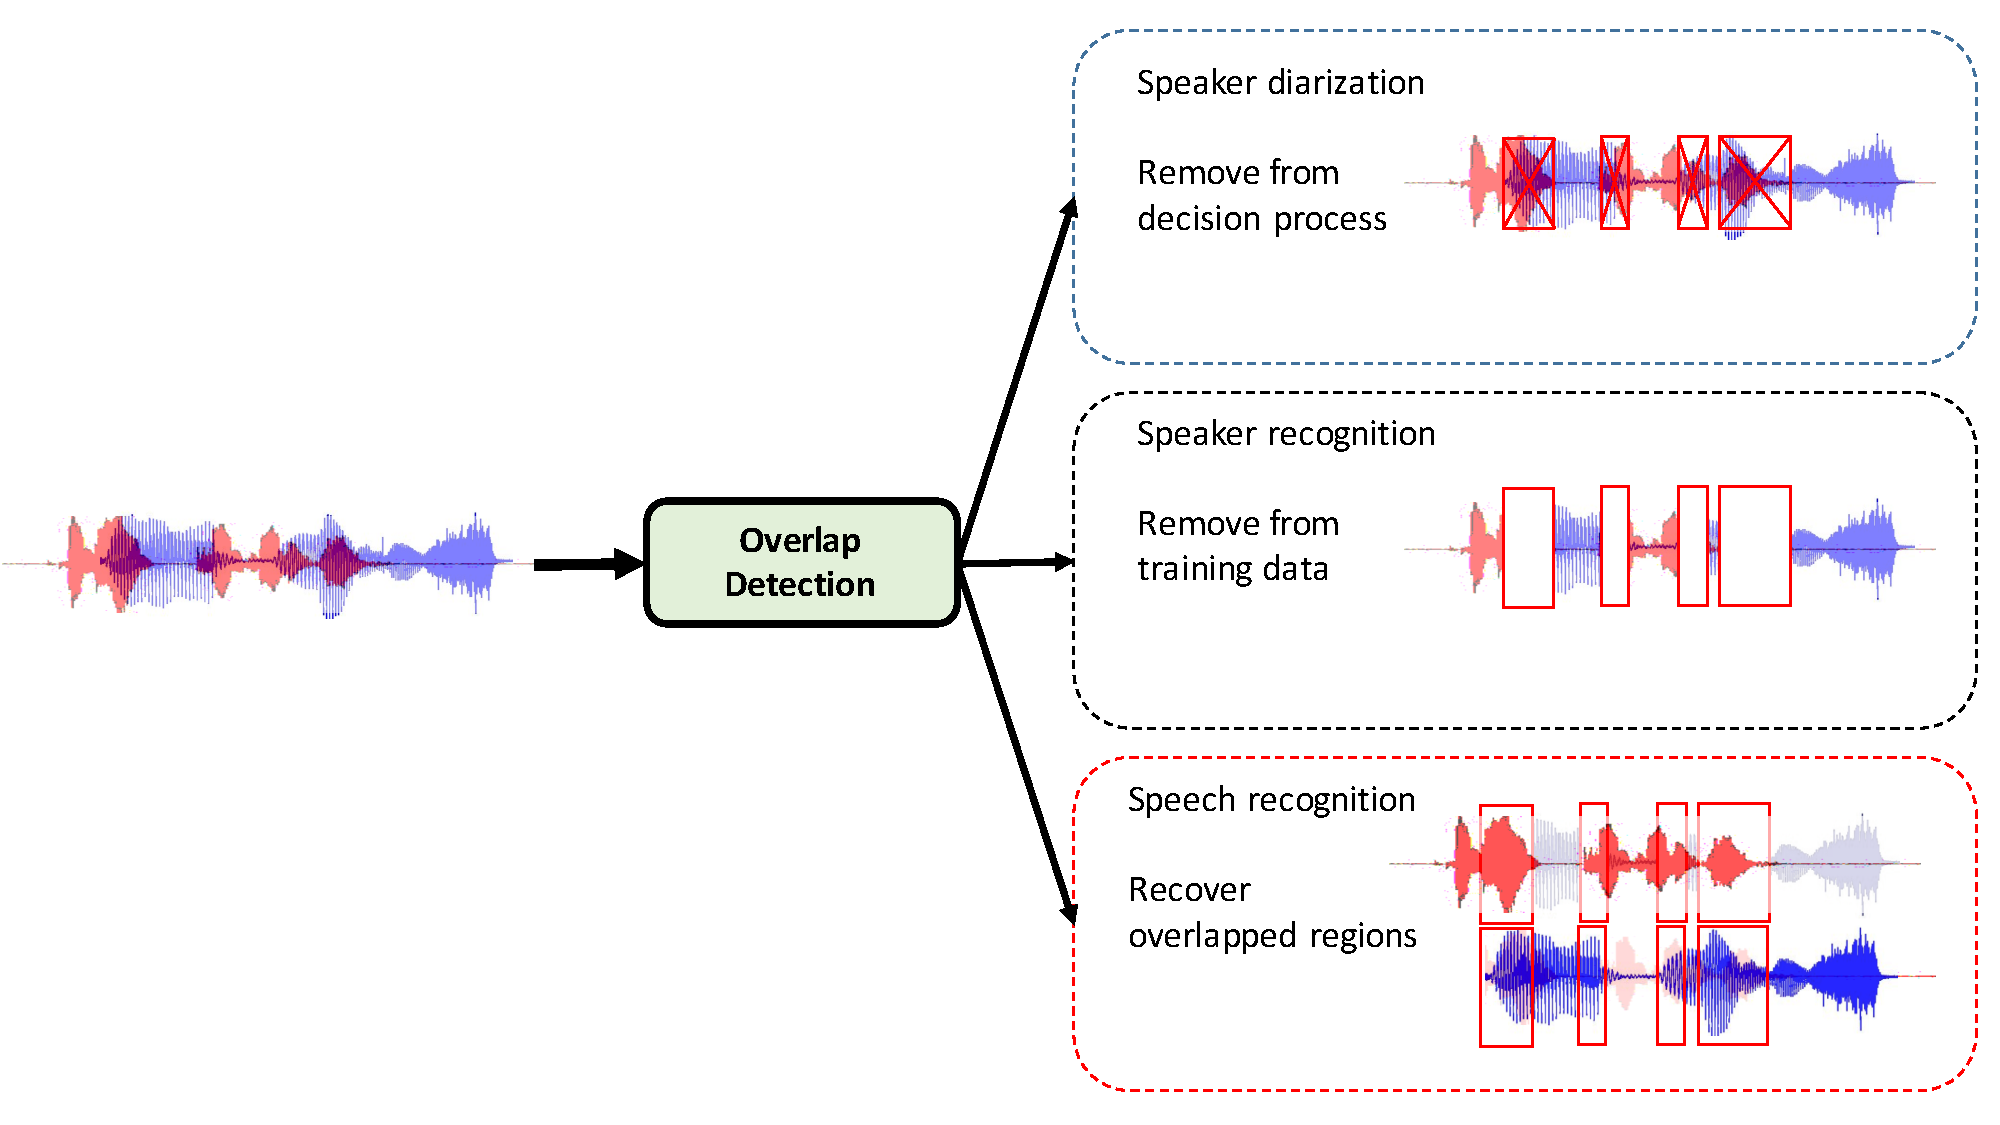
\includegraphics[height = 3in, width=0.9\textwidth]{figures/overlap_detection_applications}
	\vspace{-3mm}
	\caption{Applications of overlap detection. 
	Top: In speaker diarization, removing ignoring overlapped regions provides a more fair assessment of diarization performance. 
	Middle: Removing overlaps from in speaker recognition increases the reliability of training data.
	Bottom: Overlap detection results can be used as an initial step to recover overlapped regions.}
	\label{fig:pykno_blockdiag}
	\vspace{-3mm}
\end{figure*}

Signal processing front-end solutions in our study focus solely on overlapped speech detection. 
Figure~\ref{fig:pykno_blockdiag} summarizes incorporating overlap detection in speech processing technology. 


Detecting overlapped segments has previously been considered in tasks such as speaker identification (SID) and speaker diarization~\cite{boakye_thesis,yantorno_report}. 
In such problems, the presence of a secondary speaker either decreases model reliability (in training), or introduces confusion in the decision-making process by distorting test files. 
Detecting overlaps is computationally advantageous to enhancing the desired speaker's speech when one has the luxury of neglecting overlapped data~\cite{yantorno_report}. 
As is the case for speaker recognition and diarization~\cite{Boakye_is_08}. 
By detecting overlapped speech, we are able to remove them from the training and decision-making process. 
We begin this chapter by demonstrating the effects of manipulating the amount of overlapped data in speaker verification experiments. 
This will give us an understanding of how much overlaps affect speaker identification. 
In addition, we will see how introducing overlaps to speaker verification affects train and test data separately. 


\section{Overlaps in Speaker Verification}
\label{SID_in_GRID}

In this section, in order to show the detrimental effects of adding overlapped data to speaker verification, we present a case study of speaker recognition on data from the monaural speech separation challenge~\cite{cooke20101}. 
Our experiments use $12$-dimensional MFCC features ($13$ excluding the $0^{th}$ coefficient) plus $\Delta$ and $\Delta\Delta$, which adds to a total of 36 dimensional features. 
The experiments use the Gaussian mixture model (GMM) approach where a trained speaker is model using a mixture of Gaussians and the maximum likelihood of a given test audio file is computed from the train model. 
GMM parameters are obtained through maximum a-posterior adaptation of the parameters of a speaker independent GMM (called a universal background model which is trained on a large pool of speakers). 
We only MAP adapt GMM means in our experiments. 
$512$ mixtures were used to form the Universal background model (UBM). 
This setup requires a model for the train speakers (for whom we have several recording sessions available), but for the test speakers we only use the features to compute the ML probability of the test features belonging to the corresponding train speaker in each trial. 
The figure below summarizes the speaker verification setup. 

\begin{figure*}[h!]
	\centering
	\vspace{0mm}
	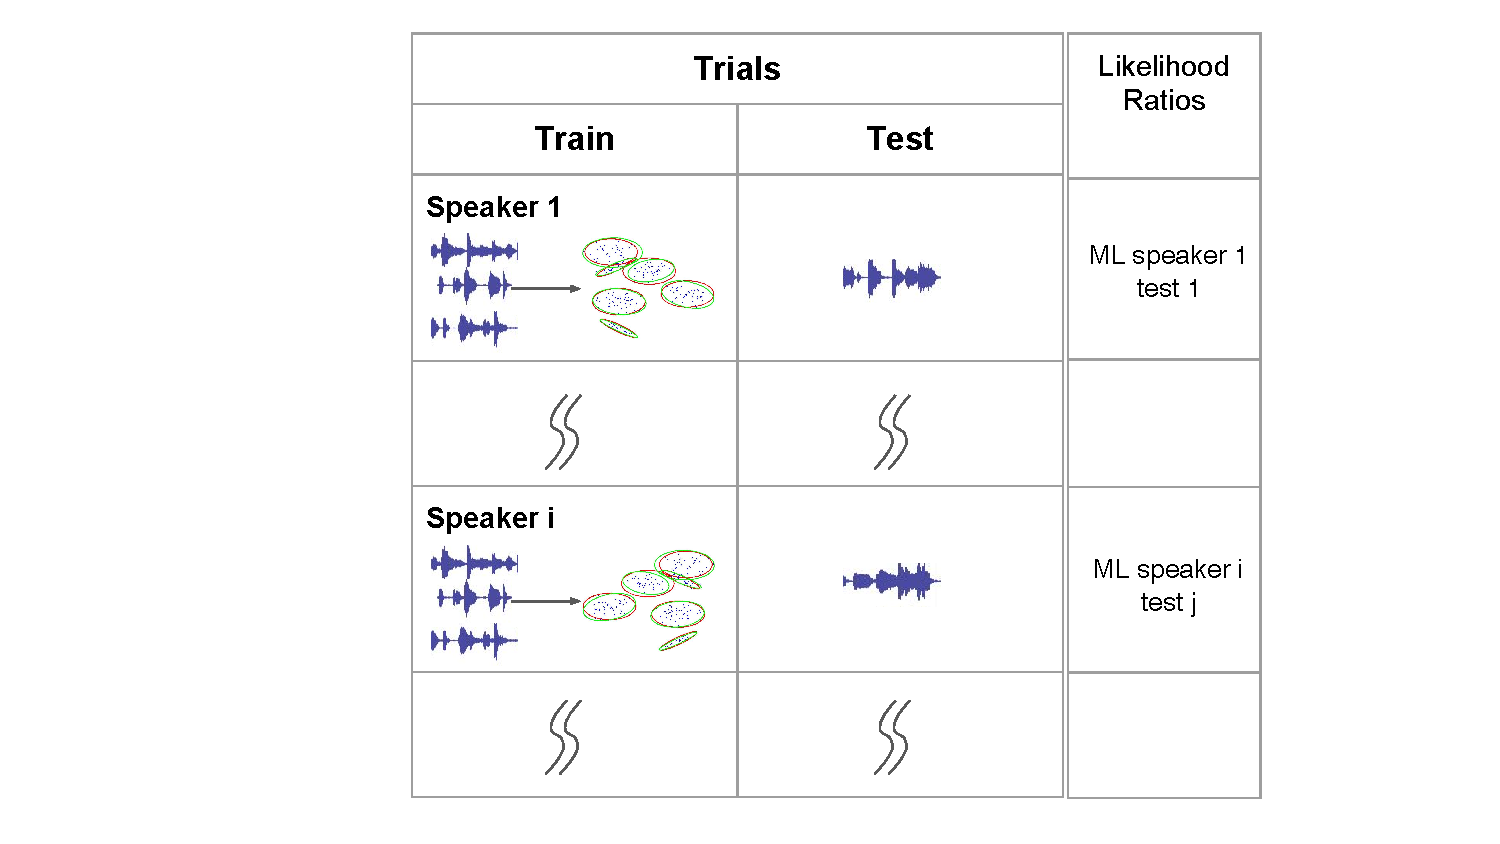
\includegraphics[height = 3in, width=0.5\textwidth]{figures/speaker_verification_setup}
	\vspace{-3mm}
	\caption{GMM-UBM speaker verification setup.}
	\label{fig:gmm_ubm_verification}
	\vspace{-3mm}
\end{figure*}


\subsection{Overlaps in test data}
As a comparison benchmark, we first evaluate SID performance under clean train and test conditions on the SSC data.
Gaussian mixture models (GMM) are adapted from a Universal back model (UBM) trained on TIMIT files~\cite{msridentity}.
For each model speaker, there are 500 utterances in SSC, which are all used in the training process. Test files are available in all SIR conditions.
As expected, lower SIR values correspond to higher equal error rates.
The presence of a secondary speaker, clearly causes confusion in the score distribution, leading to less separability between target and imposter trials.
SID performance under clean test files and those with average SIR ranging in $+6, +3, 0, -3
, -6, -9 dB$ are provided in Fig.~\ref{fig:sidingrid_ovlintest_train_a}.

It is worth mentioning that the authors were tempted to compare these results with stationa
ry noise experiments.
However, contrary to our expectations, we observed that performances were better in the ove
rlapped condition when compared to white Gaussian noise and speech-shaped noise interferenc
e, even for negative SIR values.
We find this to be a misunderstanding caused by comparing stationary and non-stationary noi
se through the same measurement procedure, which is the SIR (or SNR).
For a given target speech file, adding a certain amount of stationary noise will affect all frames, whereas in the case of non-stationary noise (here speech) only a portion of the frames receive non-uniform interference.
This leads to incomparable results under presumably similar conditions which we decided to exclude from this study to avoid confusion.

%\begin{figure*}[t!]
%	\centering
%	\begin{subfigure}[t]{0.5\textwidth}
%		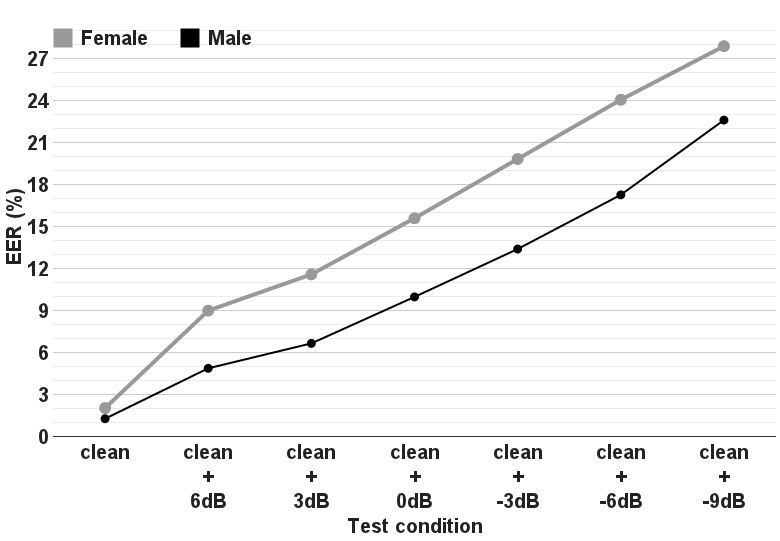
\includegraphics[width=\textwidth]{figures/sidingrid_ovlintest}
%		\vspace{-1mm}
%		\caption{~}
%		\label{fig:sidingrid_ovlintest_train_a}
%	\end{subfigure}%
%	~ %add desired spacing between images, e. g. ~, \quad, \qquad, \hfill etc.
%	%(or a blank line to force the subfigure onto a new line)
%	\begin{subfigure}[t]{0.5\textwidth}
%		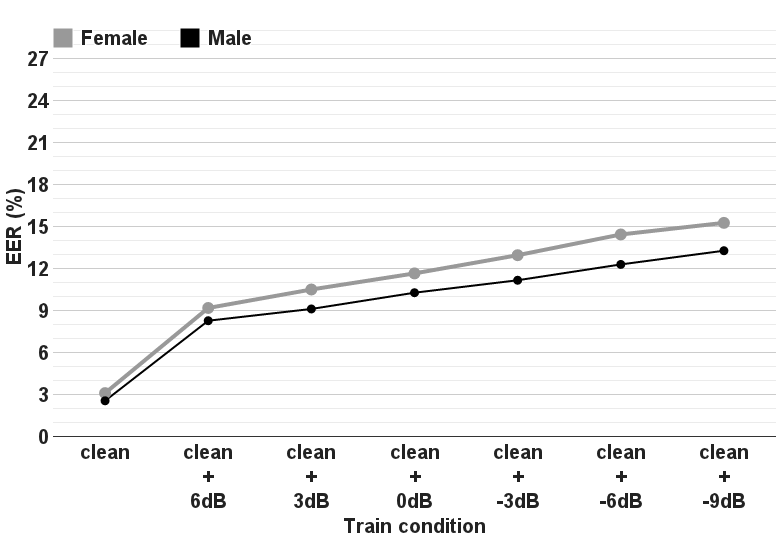
\includegraphics[width=\textwidth]{figures/sidingrid_ovlintrain}
%		\vspace{-1mm}
%		\caption{~}        \label{fig:sidingrid_ovlintest_train_b}    \end{subfigure}    \vspace{-3.6mm}
%	\caption{The rise in EER values as we increase the effect of overlapped speech (via decreasing the SIR). Starting from clean (i.e. single-speaker speech) to lower SIR values. a) Shows the case where train files are clean, but test files contain overlaps.  b) clean test files but train files contain overlaps.}
%	\vspace{-1.2mm}
%\end{figure*}
%
%\begin{figure}[!t]
%	\vspace{2mm}
%	%\centering
%	\begin{subfigure}[b]{0.3\textwidth}
%		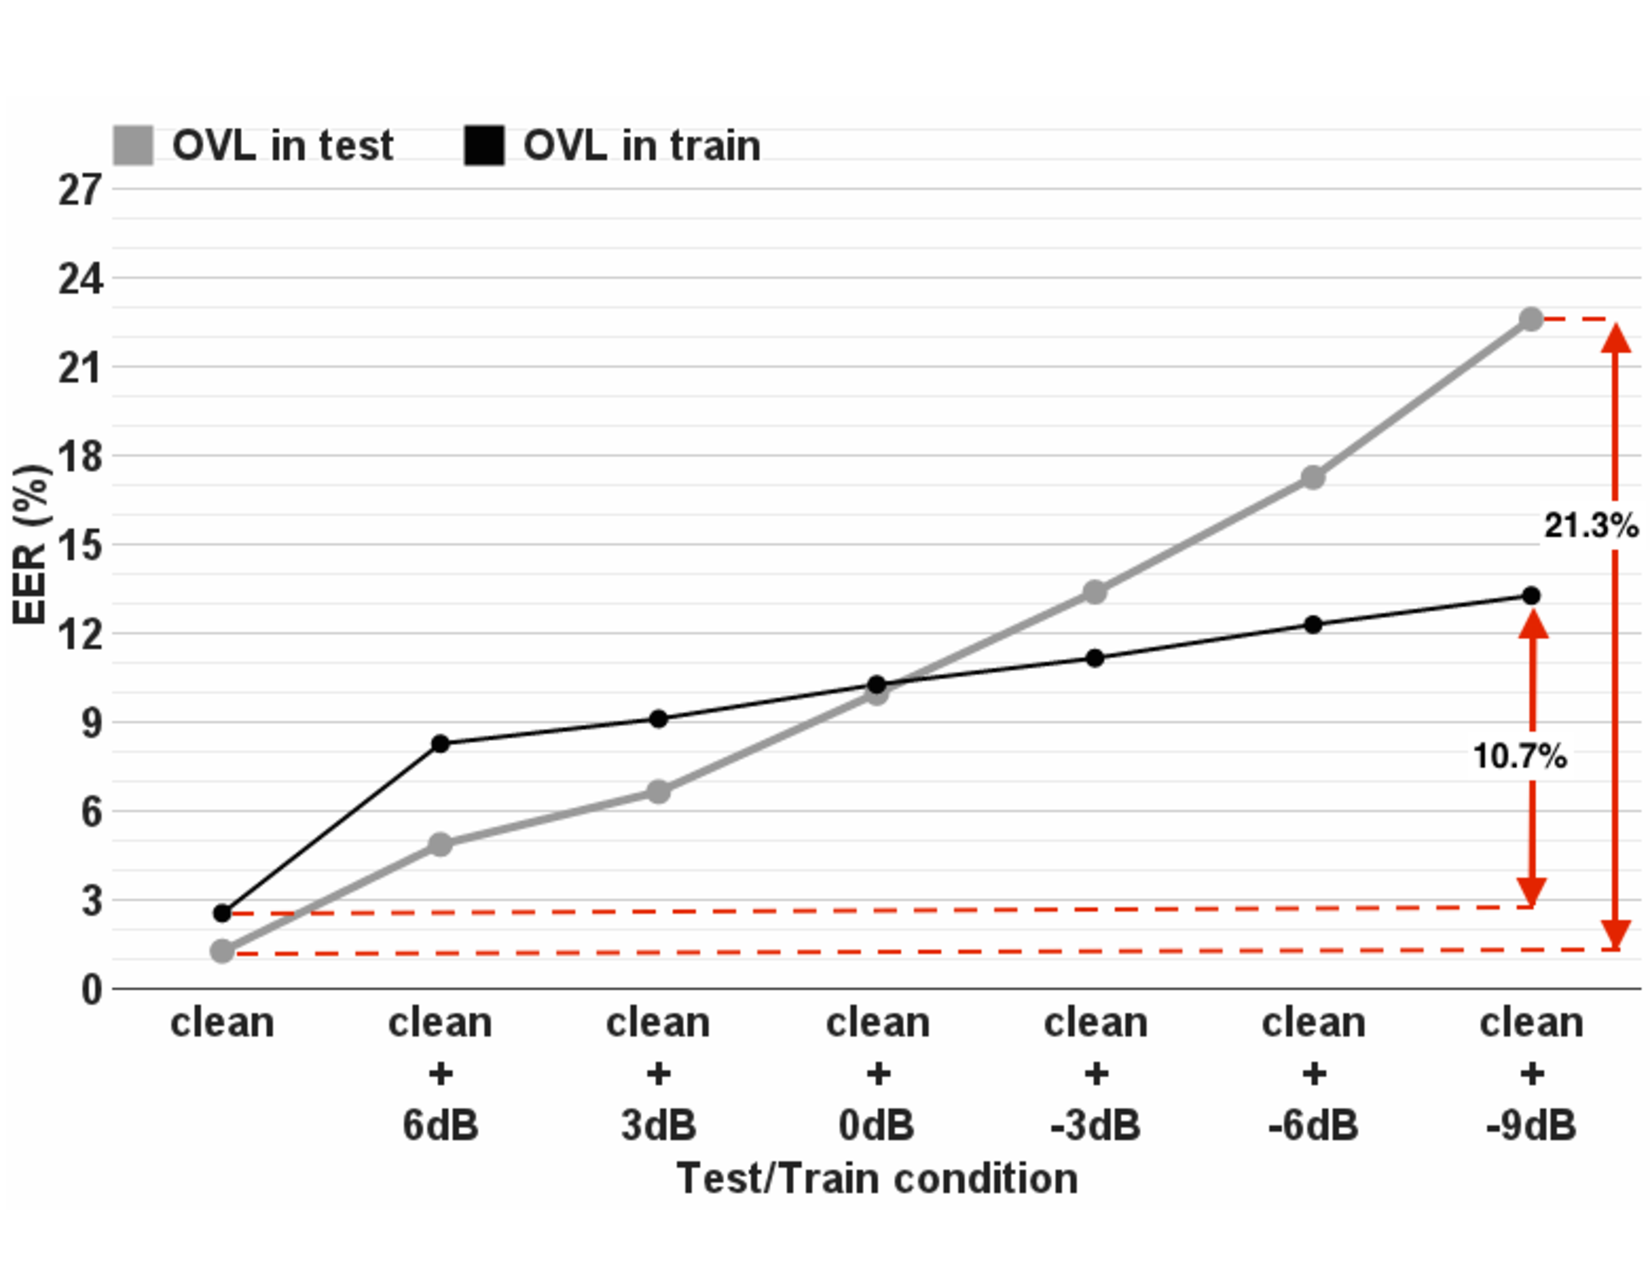
\includegraphics[height = 2.43in, width=1.6\textwidth]{figures/sidingrid_ovlintrainvstest_male_rev1}
%		\caption{male}
%		\label{fig:sidingrid_ovlintrainvstest_male}
%	\end{subfigure}
%	\begin{subfigure}[b]{0.3\textwidth}
%		\hspace{0.7\textwidth}
%		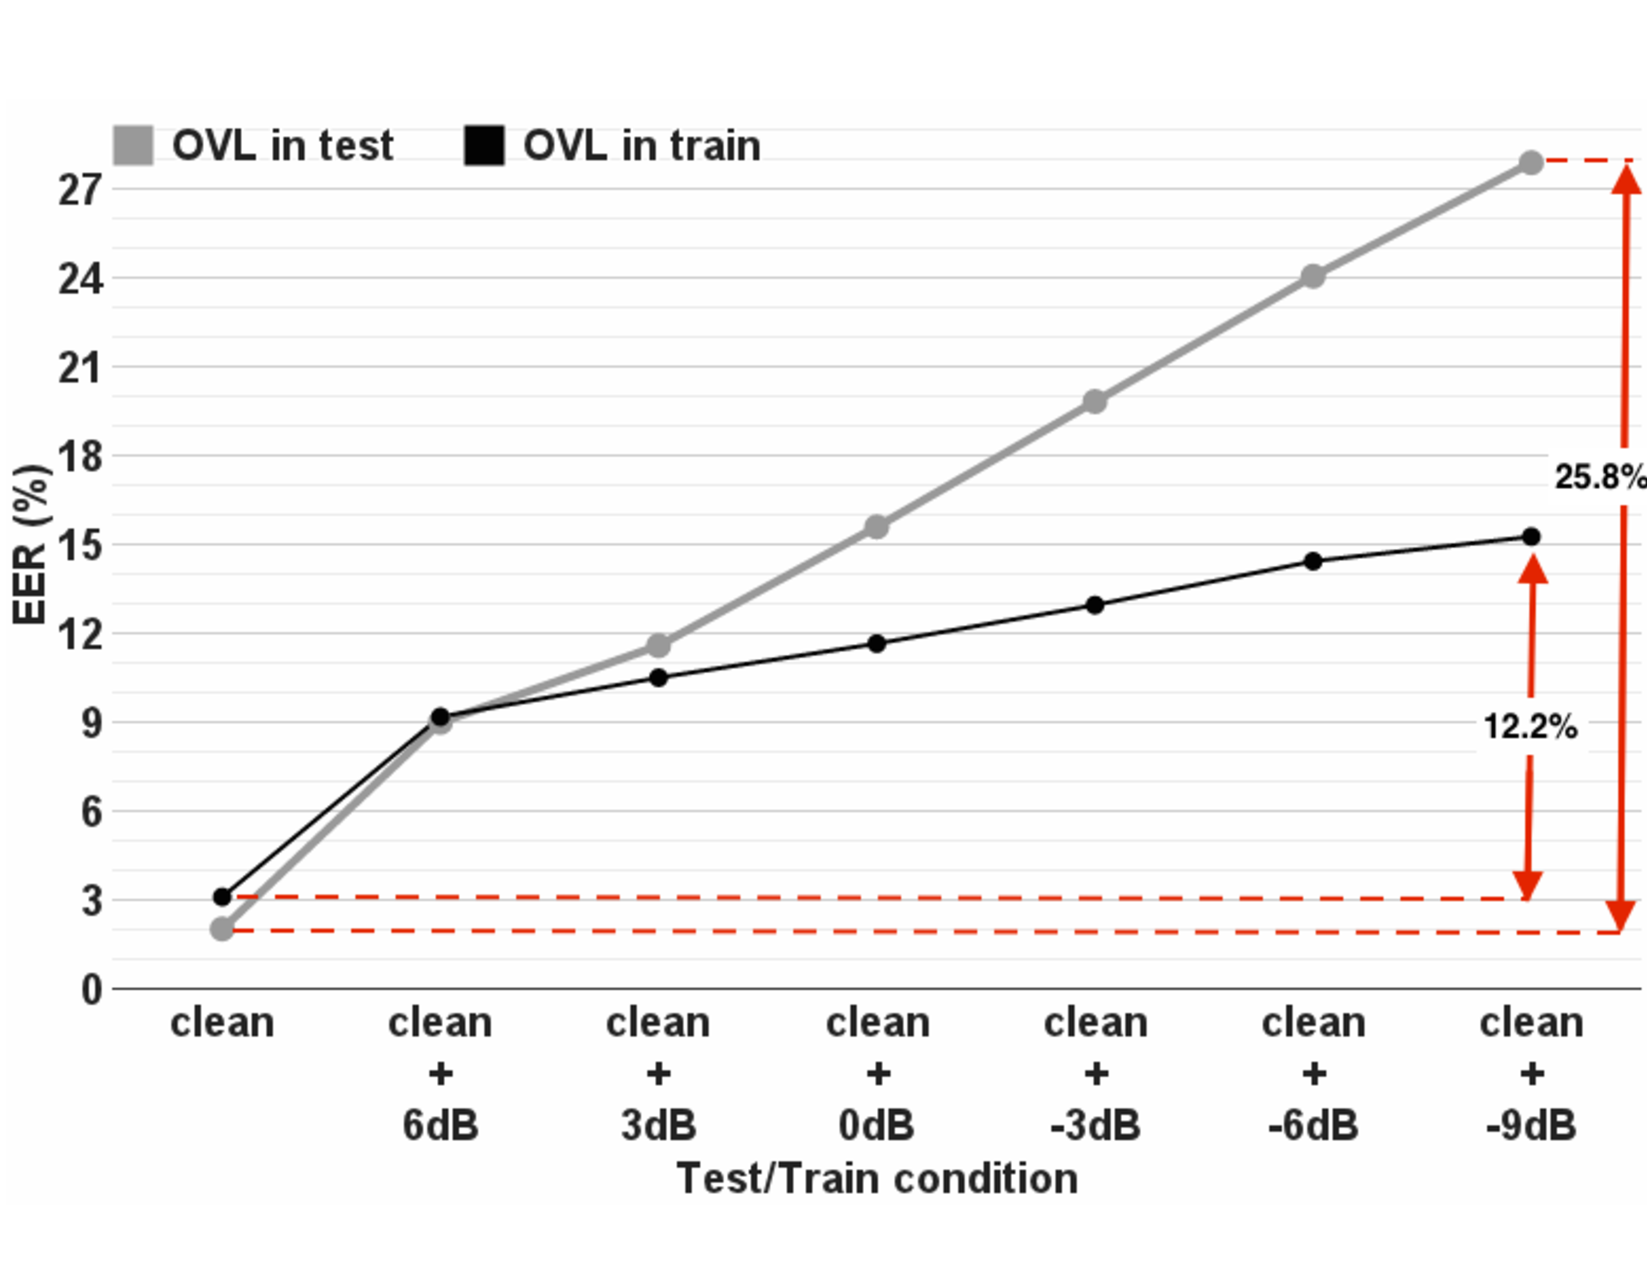
\includegraphics[height = 2.43in, width=1.6\textwidth]{figures/sidingrid_ovlintrainvstest_female_rev1}
%		\caption{female}
%		\label{fig:sidingrid_ovlintrainvstest_female}
%	\end{subfigure}
%	\caption{Comparing the impact of increasing overlap (OVL) in train vs. test data by decreasing SIR values. Experiments for male (a) and female (b) speakers. Lower SIR drops the performance more rapidly when applied to test data.}
%	
%	\vspace{2mm}
%\end{figure}

\subsection{Overlaps in train data}
We also examine the effect of adding overlapped speech to train files.
Figures~\ref{fig:sidingrid_ovlintrainvstest_male} and \ref{fig:sidingrid_ovlintrainvstest_female} compares the effects of adding overlapped speech in train and test files.

An interesting observation is the higher rate with which the EER increases when the SIR drops for the test condition.
We believe this is due to the fact that in train conditions, the training of Gaussian mixture models tends to cancel out the effect of the interfering speech.
For each speaker, the GMM is trained on a set of features, some of which are influenced by the desired speaker and the rest influenced by the interfering speakers.
Since multiple training files are used to model each speaker (different training files have different interfering speakers), the GMM tends to converge to a common locale in the feature space, which belongs to the speaker for whom the models are being trained.
We call this effect averaging out (or cancelling out) of the interfering speakers.
This to some extent slows the growth in EER as the data becomes noisier in train files.
Such cancellation, however, does not exist across test files.

\section{Background}

Traditionally, studies have used spectral harmonicity as a key factor in detecting overlapped speech~\cite{nav_icassp13,smolenski_tut}. 
This approach is motivated by the fact that two fundamental frequencies exist in most instances of overlapped speech which disarranges the harmonic structure observed in single-speaker speech. 
As a side-note here, we point out that most focus in overlapped speech has been at regions where both speakers produce ``voiced'' speech. In~\cite{morgan_cochannel} a classification of different types of segments in co-channel speech is presented. Figure~\ref{fig:morgan_v_uv_table} is adopted from~\cite{morgan_cochannel}. 

\begin{figure}[h!]
	\centering
	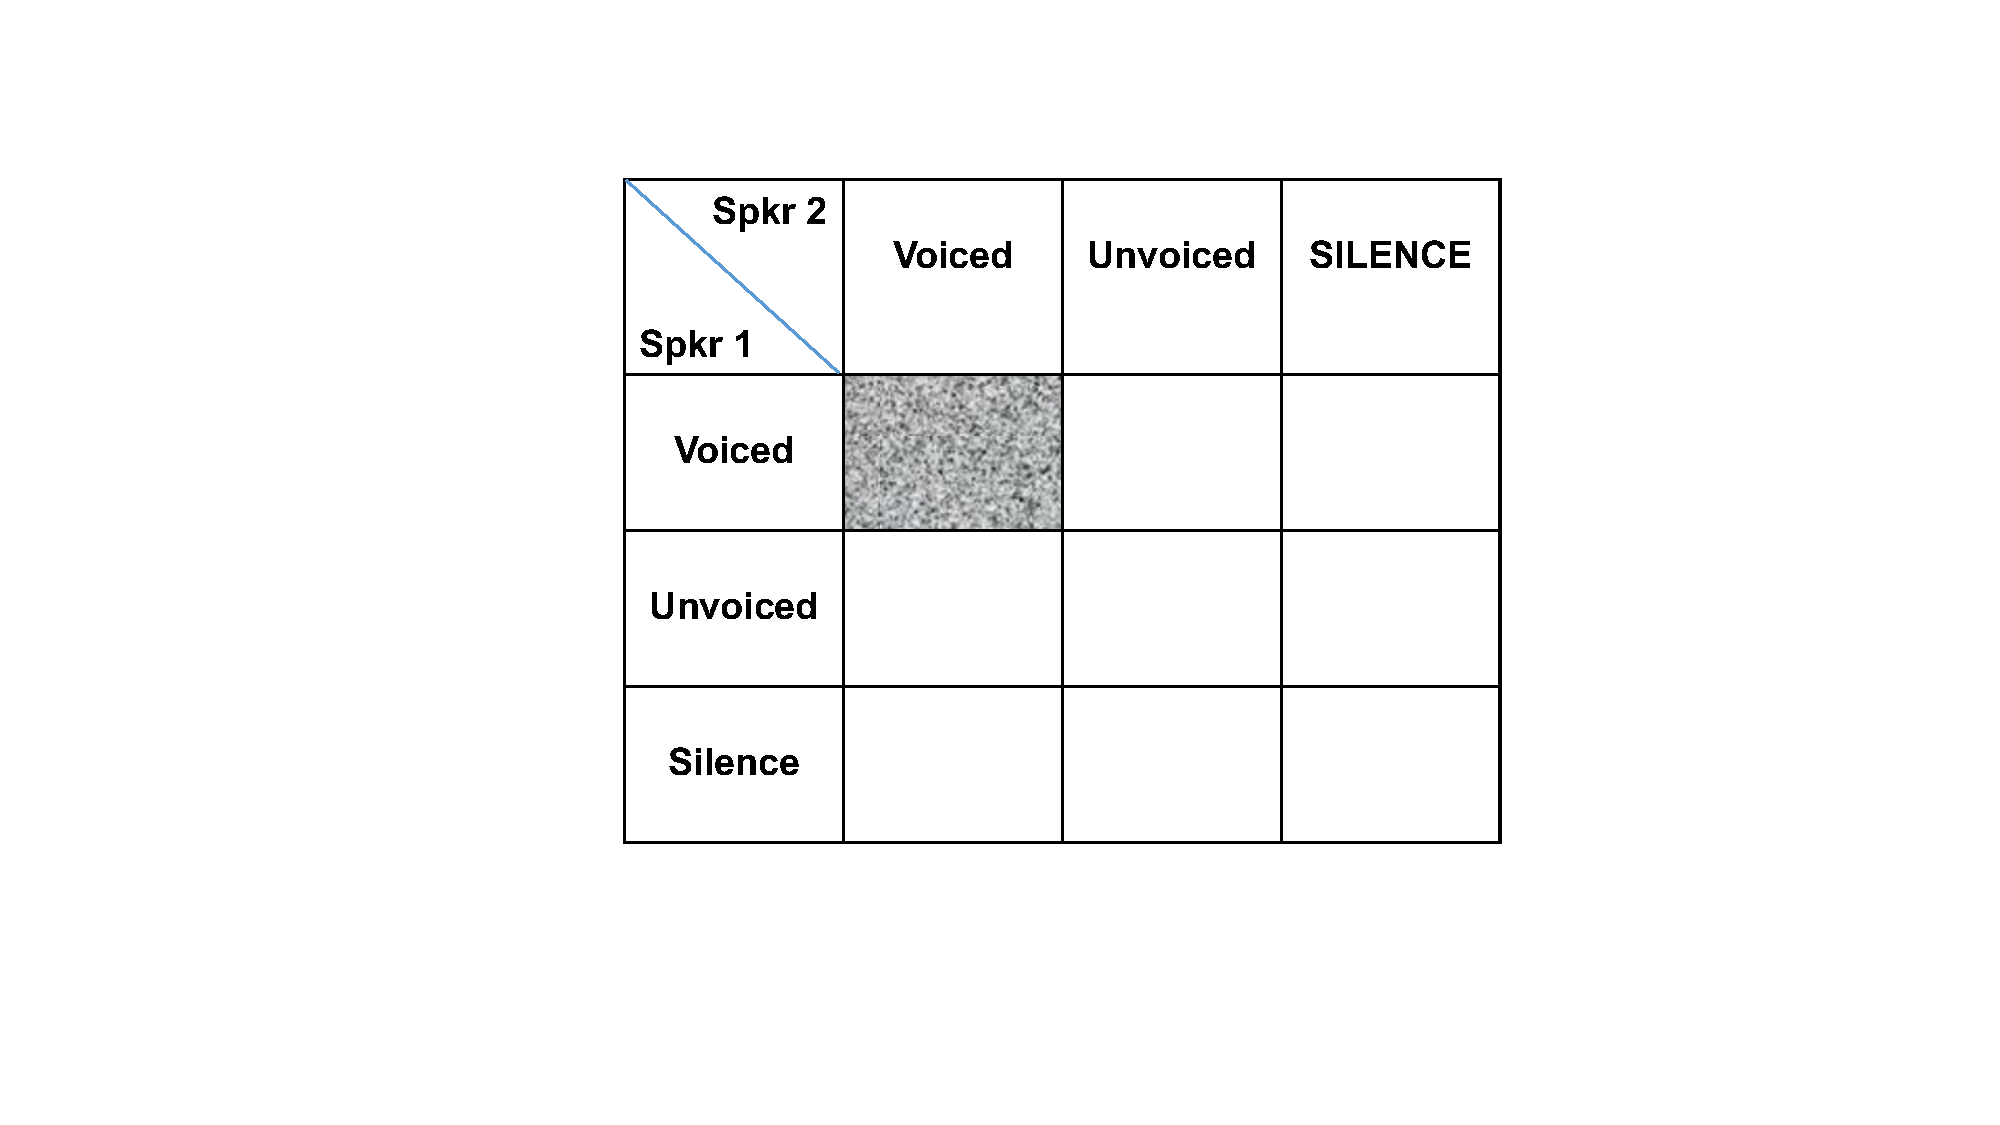
\includegraphics[height = 3.1in, width=0.5\textwidth]{figures/morgan_v_uv_table}
	\label{fig:morgan_v_uv_table}
	\caption{Classification of different segments in a co-channel file. In overlap detection we are interected in 
		the voiced-voiced (shaded) region.}
\end{figure}

Most of our focus will be on the voiced-voiced cell. 
Merely because detecting other regions becomes far more difficult. 
A more detailed classification of overlapped regions is presented in~\cite{fig:nav_icassp13}, where a grid containing all phones is used to rank-order overlapped segments in terms of difficulty. 
The analysis in~\cite{fig:nav_icasssp13} expands Fig.~\ref{fig:morgan_v_uv_table} as shown in Fig.~\ref{fig:nav_v_uv_table}. 
General consensus is to focus on detecting voiced-voiced overlap detection, which from now on we will refer to as overlap detection. 

\begin{figure}[h!]
	\centering
	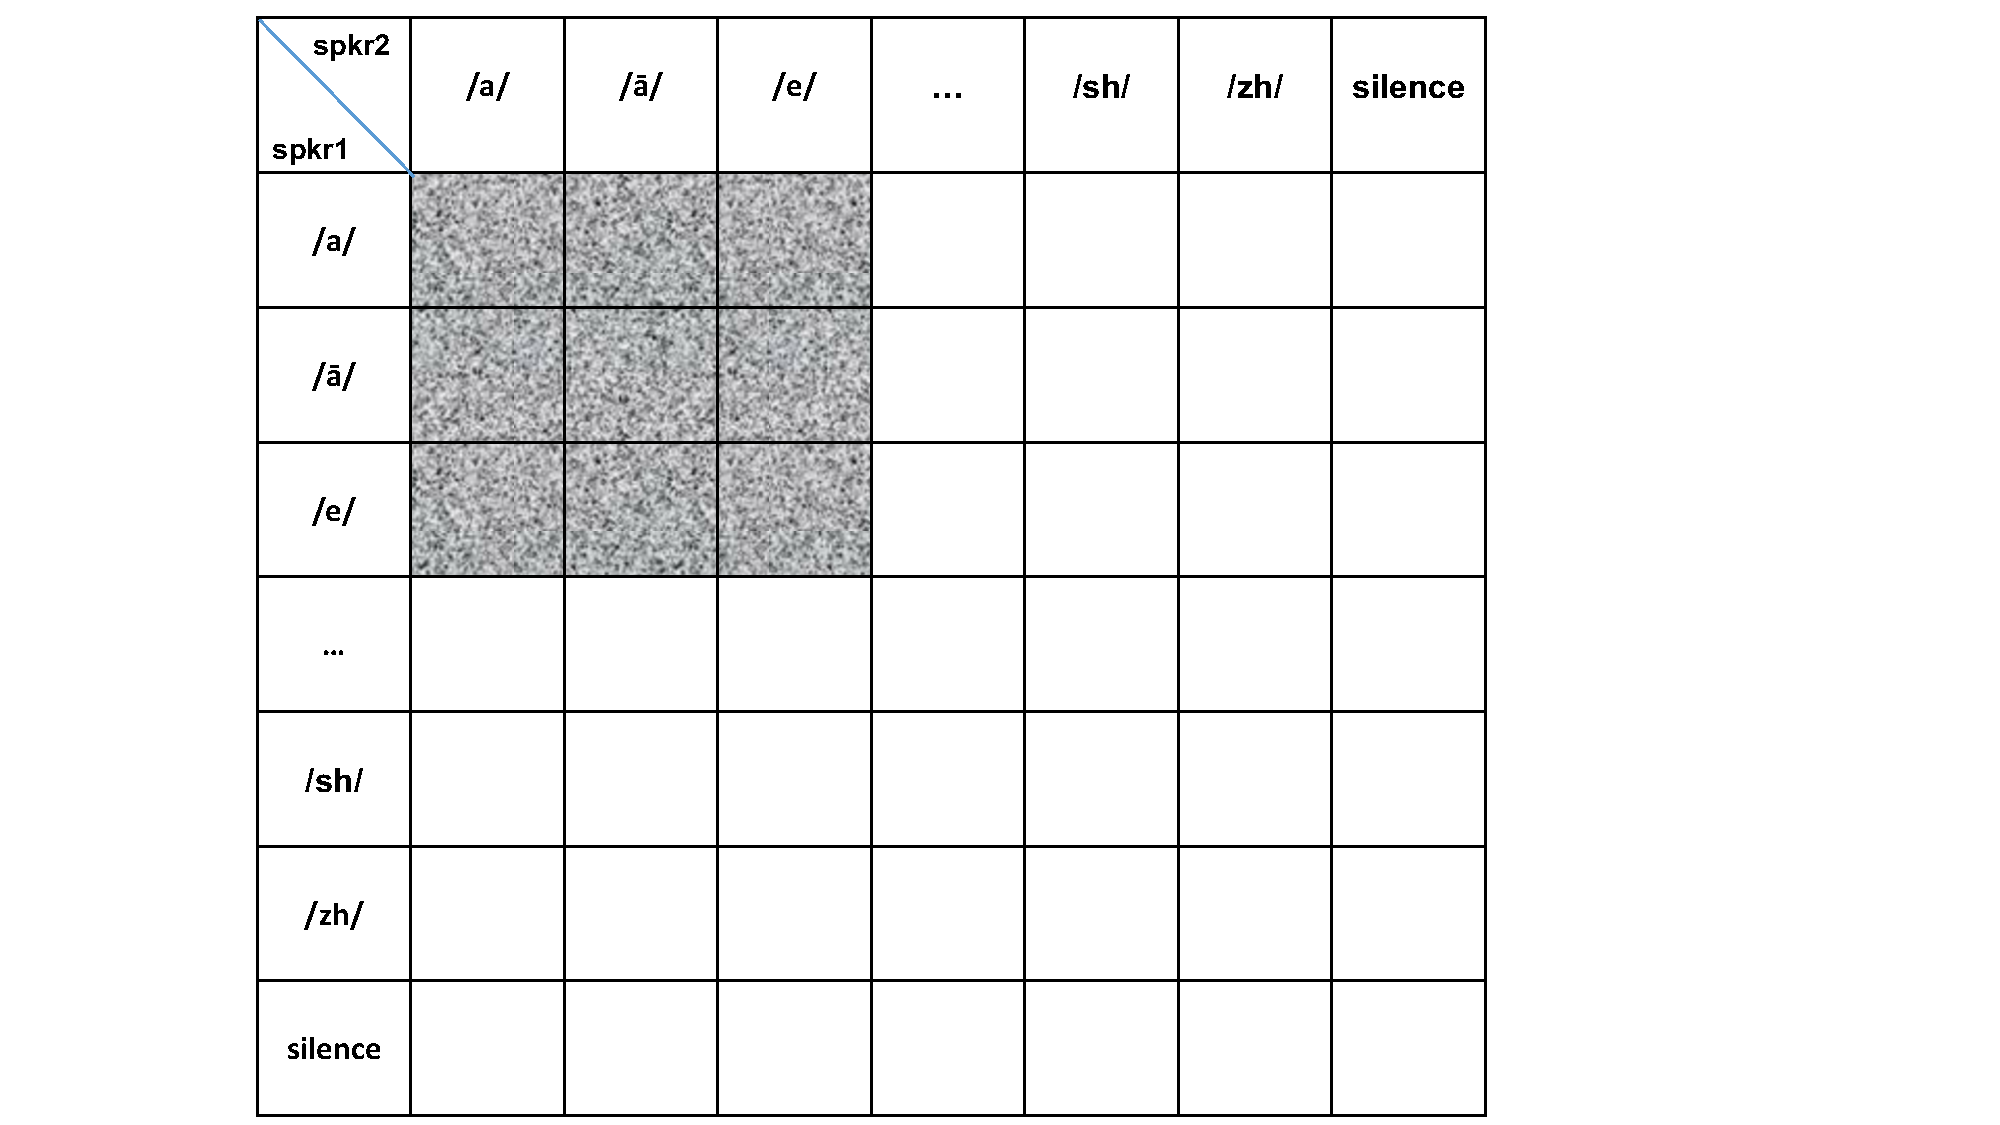
\includegraphics[height = 3.1in, width=0.5\textwidth]{figures/nav_v_uv_table}	
	\label{fig:nav_v_uv_table}
	\caption{phone-based expansion of overlapped segments in Fig.~\ref{fig:morgan_v_uv_table}.}
\end{figure}

Concentrating on voiced speech allows us to use more discriminating harmonic structures to detect overlaps. 
In~\cite{sapvr_2000}, the peak-to-valley ratios in frame-based spectral autocorrelations are introduced as a discriminating feature for overlapped speech detection through the same assumption. 
Spectral flatness measure, the ratio of geometric to arithmetic means calculated from spectral bins in a speech frame, has also been used as a measure to capture harmonicity and has been used to detect the presence of overlapped speech~\cite{nav_icassp13}. 
Another related characteristic is observed when monitoring fundamental frequencies along time. 
Adjacent pitch period comparison (APPC) presented in~\cite{appc2001} uses the temporal variation of estimated ``pitch'' periods as a measure to detect ``usable'' speech with the assumption that temporal variations of adjacent pitch periods are significantly higher in overlap. 
A multi-pitch tracking algorithm proposed in~\cite{Dwang_03_trans} was used in~\cite{Dwang_03} to estimate coexisting fundamental frequencies in the presence of multiple speakers. 
Regions where more than one fundamental frequency is estimated are labeled as overlap. 
The multi-pitch tracking technique described in~\cite{Dwang_03_trans}, decomposes speech into sub-bands and pitch estimation is only performed on reliable sub-bands. 

A slightly different, yet fundamentally similar, approach to distinguish overlapped speech is to use speech kurtosis which measures higher order moments of the signal statistics~\cite{Wrigley_05}. 


A number of studies have considered investigating spectral characteristics at formant frequency locations when dealing with overlapped speech. 
Giuliani et al. use a filter-based approach to improve speech recognition rates for different instances of meeting conditions by adding a detection step that separates double-speaker speech from single-speaker audio~\cite{giuliani_meeting}. 
This was accomplished by cascading two-layer sub-band filters to capture formant characteristics. 
Formant frequency information was obtained by filtering the signal at sub-bands with center frequencies and bandwidths corresponding to nominal ${F_1, F_2}$, and ${F_3}$ values for all English vowels. 
One of the reasons Formant-based overlapped speech analysis has received less attention is the difficulties in modeling pole interactions at overlapped regions, which is an issue for linear predictive modeling and other commonly used formant tracking techniques. 
Characterizing pole interactions using standard LP models easily becomes intractable in the presence of more than one source. 
Add to this complication, the unknown speaker locations with respect to each other and the microphone. 
As a result, we focus our attention to nonlinear speech models, some of what have proven more successful in the scenarios described above. 

Nonlinear speech models, including the AM-FM speech model~\cite{maragos_kaiser_quatieri} have been used in previous studies to model speech resonances without any specific requirements for the source signal. 
These energy operators have also been used to deal with signals with more than one source~\cite{maragos_instantaneousenergy}, aka co-channels signals~\footnote{Co-channel is a more general terminology used to described multi-component signals. 
In the case of speech, co-channel speech may refer to any single-channel recording that contains speech from multiple speakers, regardless of whether there is overlap.}. 
Maragos et al. use higher order energy operators to develop an algorithm that simultaneously demodulates the components of a co-channel mixture in AM-FM modulated signals~\cite{maragos_instantaneousenergy}. 
Litvina et al. separate speech from music using the Teager energy operator (TEO) separation algorithm~\cite{maragos_kaiser_quatieri}~\cite{Litvin2010}, where they used the extracted components to design a time-varying filter and suppress the interfering signal. 
Similar multicomponent signal decomposition techniques have been addressed using energy operators to separate narrow-band signals~\cite{Linicassp95,hu12_nullspacepersuit,santhanam_maragos_2000}. 

Our goal is to incorporate sub-band analysis to design a technique suitable for {\bf overlapped speech detection}. 
Two algorithms are proposed that incorporate sub-band analysis for overlap detection. 
\begin{itemize}
	\item using TEO methods on narrow-band components to detect speech harmonics. 
	\item apply cosine functions across sub-band outputs to magnify the presence of multiple harmonics. 
\end{itemize}


%%%%%%%%%%%%%%%%%%%%%%%%%%%%%%%%%%%%%%%%%%%%%%%%%%%%%%%%%%%%%%%%%%%%%
%%%%%%%%%%%%%%%%%%%%%%%%%%%%%%%%%%%%%%%%%%%%%%%%%%%%%%%%%%%%%%%%%%%%%
%%%%%%%%%%%%%%%%%%%%%%%%%%%%%%%%%%%%%%%%%%%%%%%%%%%%%%%%%%%%%%%%%%%%%
%%%%%%%%%%%%%%%%%%%%%%%%%%%%%%%%%%%%%%%%%%%%%%%%%%%%%%%%%%%%%%%%%%%%%

\section{Pyknograms}
\label{sec:ovldet}

We propose a novel approach for overlapped speech detection based on an enhanced spectrogram. 
These spectrograms, called Pyknograms, were first introduced by Potamianos and Maragos in~\cite{potamianos_maragos_icassp95,potamianos_maragos_jasa96} and are calculated by applying multi-band demodulation in the AM-FM speech model framework~\cite{maragos_kaiser_quatieri}{\footnote{The authors in~\cite{potamianos_maragos_jasa96} used the term ``Pyknogram'' which stems from the Greek word ``pykno'' meaning dense. Pyknograms represent highly resonating regions in time-frequency plots as populated scatter plots, hence the term density.}. 
Pyknograms provide a more prominent representation of harmonic trajectories, which we propose to use as a means to detect the presence of interfering speech.


\subsection{Energy Operators and the AM-FM speech model}

In Pyknograms~\cite{potamianos_maragos_jasa96}, the harmonic structure of speech is enhanced by decomposing spectral sub-bands into amplitude and frequency components. 
This multi-band analysis uses the AM-FM speech model~\cite{maragos_kaiser_quatieri} to decompose sub-bands and thereby calculate corresponding instantaneous frequencies and bandwidths: (\ref{eq:instamp}),~(\ref{eq:instfreq}). 
Pyknogram extraction locates dominant peaks in the spectrogram from instantaneous frequencies. 
To extract Pyknograms, the speech signal is initially passed through a filter-bank (we have modified the algorithm to use logarithmically spaced Gamma-tone filters, while~\cite{potamianos_maragos_jasa96} uses linearly-spaced Gabor filters). 
Filter-bank outputs are then decomposed into amplitude and frequency components using the discrete energy separation algorithm (DESA-1)~\cite{maragos_kaiser_quatieri}, where the frequency and amplitude components of a given sub-band, $x(n)$, are calculated using the discrete energy operator,
 

\begin{equation}
\Psi [x(n)] = x^2(n)-x(n-1)x(n+1),
\end{equation}
$\Psi [x(n)]$ is energy operator used to estimate amplitudes and instantaneous frequencies, as shown in Fig.~\ref{fig:desa1}. 


\begin{equation}
\label{eq:instfreq}
f(n) = \frac{1}{2\pi}\arccos \Big (1-\frac{\Psi[x(n)-x(n-1)]}{2\Psi[x(n)]}\Big),
\end{equation}
 
 
\begin{equation}
\label{eq:instamp}
|a(n)| = \sqrt{\frac{\Psi[x(n)]}{\sin^2(2\pi f(n))}}.
\end{equation}



\begin{figure}[b]{3.5in}
	\centering
	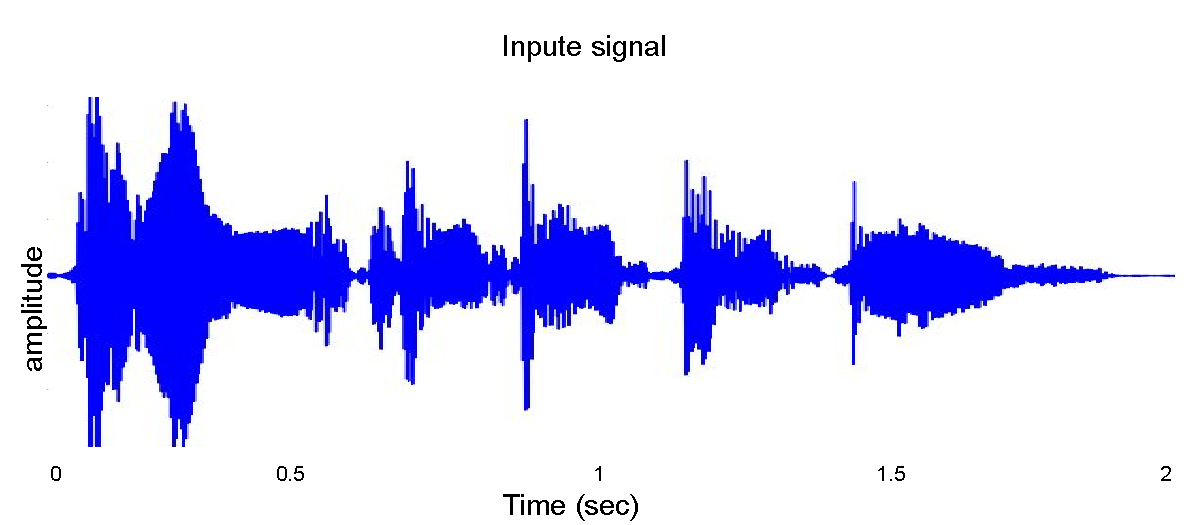
\includegraphics[height=1.5in, width=4in]{figures/teo_signal}
	\caption{Input signal.}
\end{figure}
	
\vspace{1.0mm}
\begin{figure}[b]{3.5in}
	\centering
	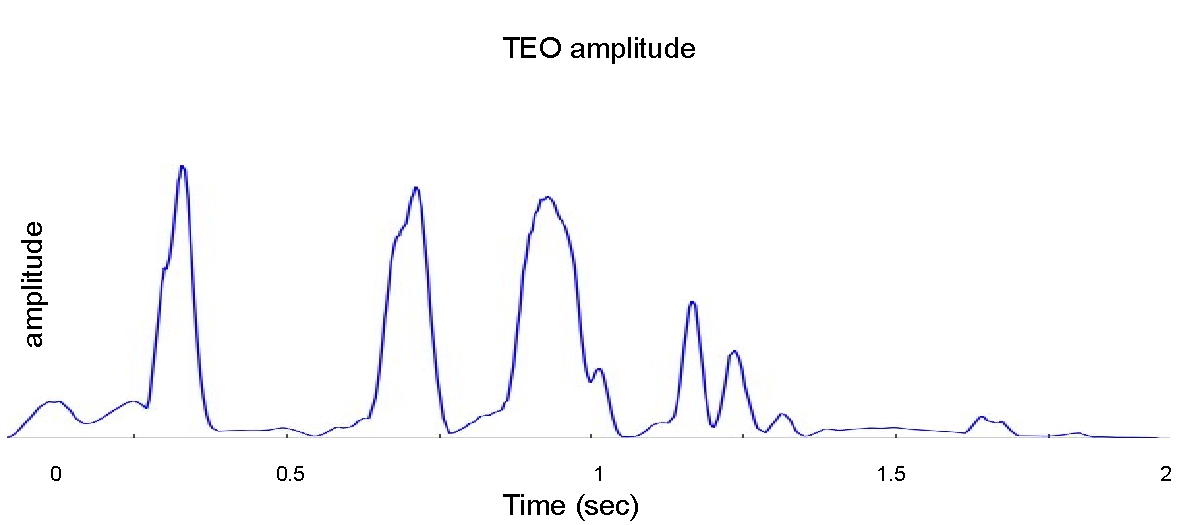
\includegraphics[height=1.5in, width=4in]{figures/teo_amp}
	\caption{Outputs of DESA-1: Signal amplitude component estimated using TEO, Eq.~(\ref{eq:instamp}).}
\end{figure}

\begin{figure}[b]{3.5in}
	\centering
	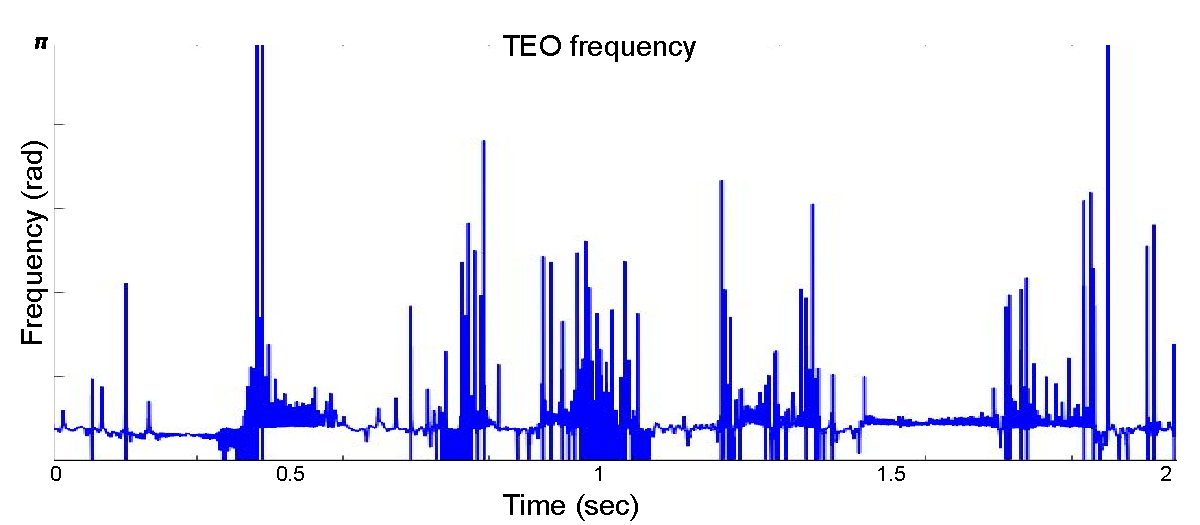
\includegraphics[height=1.5in, width=4in]{figures/teo_freq}
	\caption{Outputs of DESA-1: Signal frequency component estimated using TEO,  Eq.~(\ref{eq:instfreq}).}
\end{figure}

\subsection{Pyknogram Extraction}
\label{ssec:pyknogram_extraction}

Pyknograms are estimated from DESA-1 outputs. The weighted average of instantaneous frequency components (see~(\ref{eq:weighted_f})) is used to derive a short-time estimate of the dominant frequency in each sub-band over time-frame units (typically 25 msec)~\cite{cohenlee90}. 
Frequencies are weighted using the estimated signal power ($|a(n)|^2$). 
The average frequency computed for each frame/sub-band (time-frequency unit) can be viewed as the $1^{st}$-order moment of instantaneous frequencies.  


\begin{equation}
\label{eq:weighted_f}
F_w(t) = \frac{\sum_{t}^{t+T}f(n)a^2(n)}{\sum_{t}^{t+T}a^2(n)},
\end{equation}
The algorithm also provides a means to estimate weighted bandwidths for each resonance, (\ref{eq:weighted_bw}). 
What we refer to here as bandwidths are essentially $2^{nd}$-order frequency moments. 

\begin{equation}
\label{eq:weighted_bw}
B_w(t) = \sqrt{\frac{\sum_{t}^{t+T}(\overset{\boldsymbol .}{a}(n) /2\pi)^2+(f(n)-F_w)^2a^2(n)}{\sum_{t}^{t+T}a^2(n)}},
\end{equation}
where $f(n)$ and $a(n)$ are instantaneous frequency and amplitude values from (\ref{eq:instfreq}) and (\ref{eq:instamp}). 
In (\ref{eq:weighted_f}), the instantaneous frequencies are averaged over the $t^{th}$ frame using squared instantaneous amplitudes as weights. 
$T$ in (\ref{eq:instfreq}) is the number of samples per frame, from $n = t$ to $n = t+T$. 
$\overset{\boldsymbol .}{a}(n)$ is the first difference of $a(n)$ (i.e., $a(n) - a(n-1)$). 
The per-frame values of $F_w$ provide initial estimates of spectrogram peaks. 
This results in a time-frequency {$t$-$f$} representation of the overall signal, where time units correspond to frames and frequency units to filter-bank sub-band indexes. 


In~\cite{potamianos_maragos_jasa96}, the bandwidth values defined in (\ref{eq:weighted_bw}) are used for analysis purposes. 
Here, we use them in overlap detection systems to determine the reliabilitiy of $t-f$ units. 
Our assumption is that large Pyknogram bandwidths correspond to higher uncertainty in frequency estimates. 
We investigate this in following sections by adding an uncertainty term to our frequency estimate proportional to the estimated bandwidth:



\begin{equation}
\label{eq:jitter_f}
\tilde F_w(t) = F_w(t) + \epsilon_t,
\end{equation}
where
\begin{equation}
\label{eq:jitter_pdf}
\epsilon_t \sim\ \mathcal{N}(0,B_w(t)).
\end{equation}

As a final step, dominant harmonic peaks are selected by comparing the average frequency estimates with filter-bank center frequencies. 
According to~\cite{potamianos_maragos_jasa96}, points at which filter-bank center frequencies coincide with the weighted frequency estimates from (\ref{eq:weighted_f}) are more reliable in estimating spectrogram peaks. 
The assumption being that frequency estimates are more accurate when aligned with a filter in the filter-bank. 
This defines the condition through which initial $F_w$ values are tested to detect whether they correspond to prominent peaks. At frame $t$: 
\vspace{0mm}
\begin{equation}
\label{eq:RF1}
F_w(c) = c  \quad \iff \quad \{c \in peaks\}
\vspace{1mm}
\end{equation}
where $c$ are the filter-bank center frequencies. 
Note that center frequencies are distributed in a logarithmic scale. 
Another peak selection condition (as shown in Fig.~\ref{fig:pykno_blockdiag}) is to limit the relative variance of selected frequencies with respect to center frequencies. 

\begin{equation}
\label{eq:RF1}
\frac{\partial F_w(c)}{\partial c} < thr
\vspace{1mm}
\end{equation}
This condition limits non-harmonic anomalies that break the patterns in regular speech trajectories. 
Since such patterns are frequently observed in overlapped data, we omit this restriction from the peak-picking step.  

\begin{figure*}[t!]
	\centering
	\vspace{0mm}
	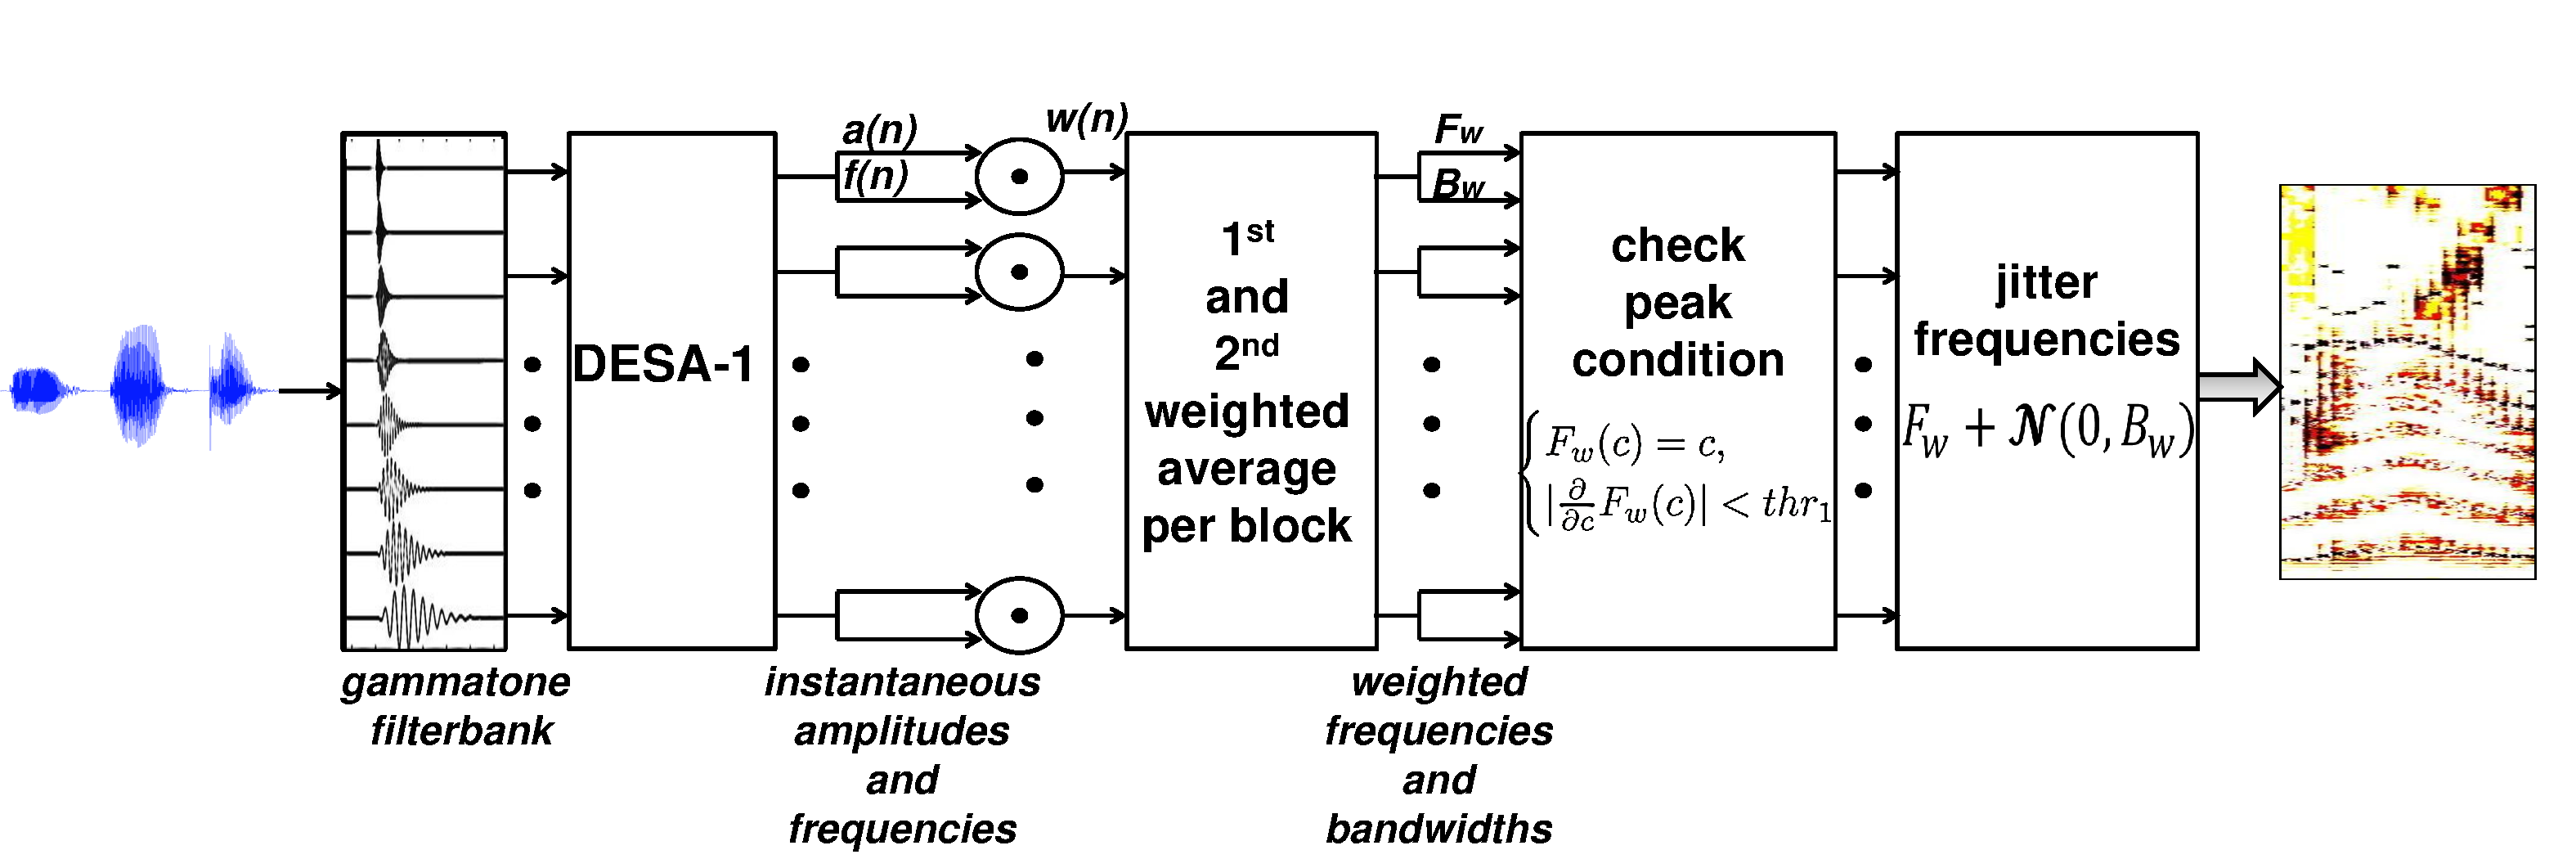
\includegraphics[height = 2.5in, width=1\textwidth]{figures/pyknogram_blockdiagram}
	\vspace{-3mm}
	\caption{Pyknogram extraction block-diagram.}
	\label{fig:pykno_blockdiag}
	\vspace{-3mm}
\end{figure*}


One of the advantages of the peak-picking constraint in (\ref{eq:RF1}) is the quantization of spectrograms onto filter-bank center frequencies. 
This allows the mapping of all signals onto a unified space defined by the filter-bank, which enables reliable comparison within the time-frequency space. 

Using an energy operator based approach helps avoid assumptions on the number of speakers in the signal. 
AM-FM decomposition is suitable since it relies on signal resonances and does not restrict signals to a specific structure or number of speakers (as opposed to models such as linear prediction). 
The final time-frequency representation is called a Pyknogram and is denoted $S_{pyk}(t,f)$ as a function of time ($t$) and frequency ($f$). 
Using Pyknograms, we would like to investigate overlap detection methods.

%\subsection{Detecting overlapped segments from Pyknograms}
Discontinuities in the Pyknogram layout is an indication of interfering speech. 
An analogy for speech harmonic patterns are skiing tracks left behind on a snowy surface. 
In the single-speaker case, the patterns leave parallel tracks that progress relatively slowly over time and correspond to fundamental frequency harmonic tracks. 
In the presence of an interfering speaker, these patterns are distorted by similar but intersecting tracks, which adds sudden jumps along the time axis (as shown in Fig.~\ref{fig:pyknograms_for_overlaps}). 
Since the majority of speakers are only capable of producing one fundamental frequency at each time instance, it is expected that the harmonic tracks should be consistent across time. 
This keeps harmonics parallel over short time intervals.   
The presence of a second speaker creates harmonic tracks that in general do not follow the same patterns, hence discontinuities are observed along time in Pyknograms. We use variations across adjacent frames as our measure of overlapped speech.

\begin{figure}[h!]
	\centering
	\vspace{4mm}
	\textbf{Pyknogram}\par\medskip
	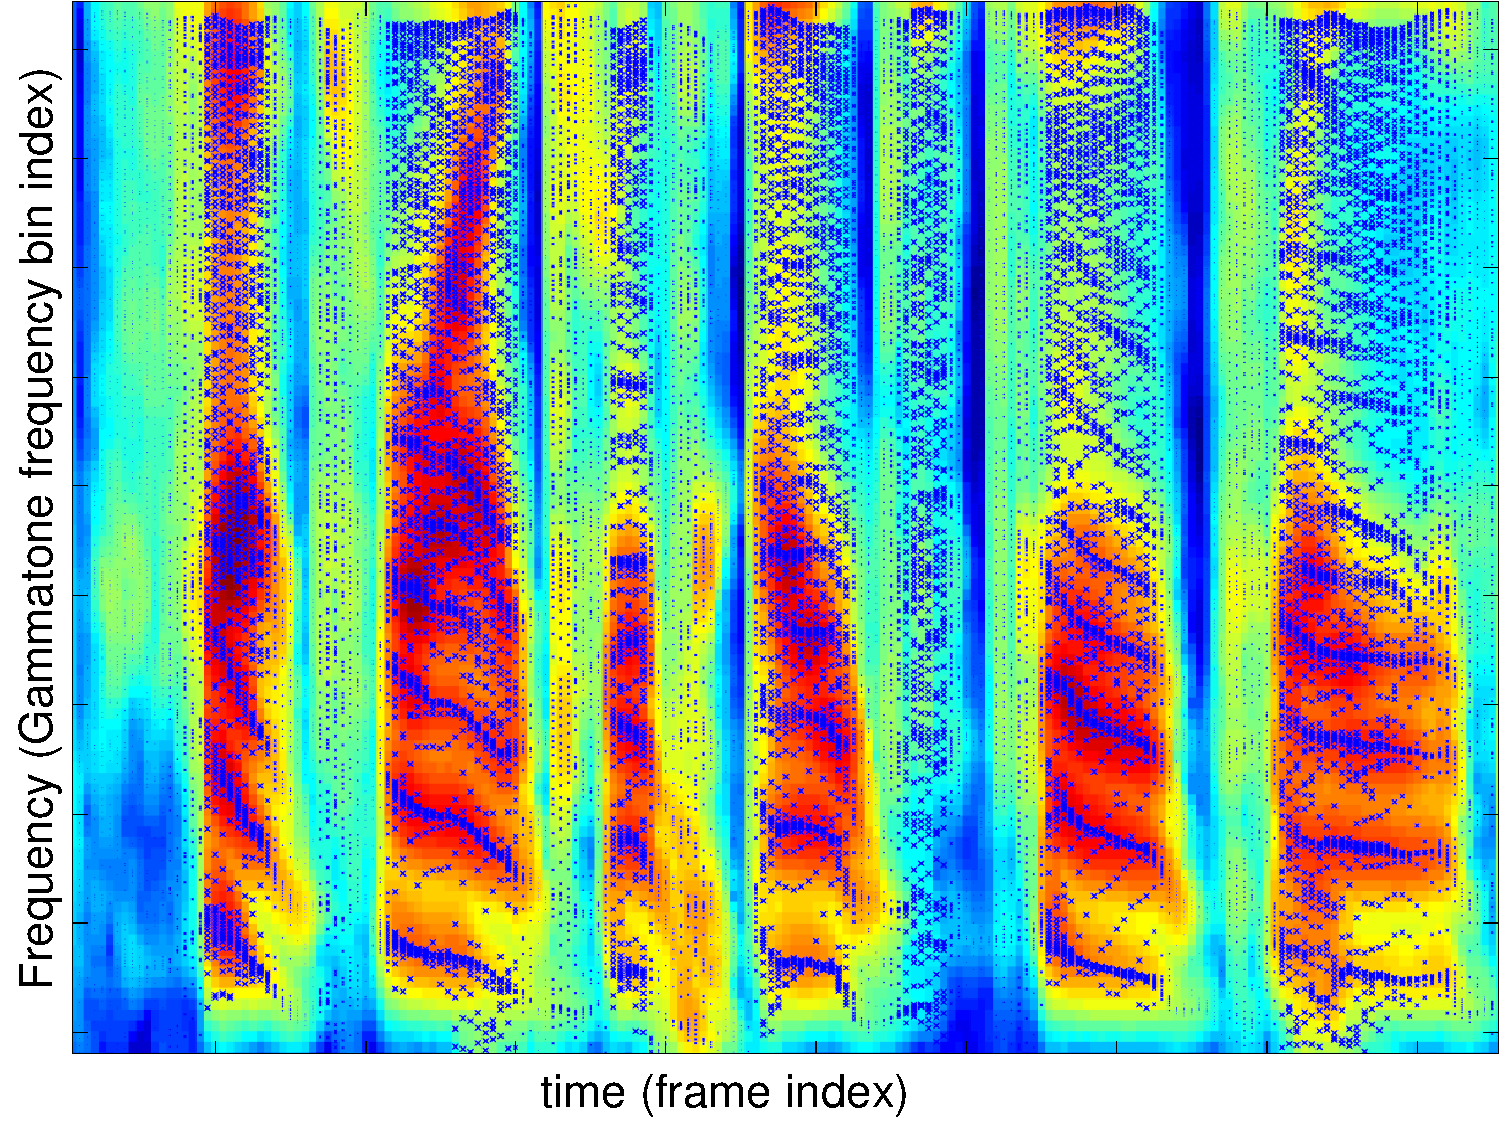
\includegraphics[height =3.in, width=0.8\textwidth]{figures/pyknogram_vs_spectrogram}
	\vspace{-1mm}
	\caption{Pyknogram for a given speech signal. The spectrogram is plotted in the background for comparison. Pyknogram markers have been scaled by the amplitudes of corresponding $t$-$f$ units. Frequencies are scaled to equivalent rectangular bandwidth (ERB) rate.}
	\vspace{-1mm}
	\label{fig:pyknograms}
\end{figure}

\subsection{Unsupervised overlap detection Pyknograms}

The average Euclidean distance between consecutive frames across all frequencies can be used to detect sudden jumps in Pyknograms along time. 
Similar to the technique used for spectral flux estimation~\cite{Rossignol_spectralflux}. 
The distance function, $D_{ovl}$, at frame $t$ is computed as the $2$-$norm$ distance between consecutive Pyknogram frames, $S_{pyk}(t,f)$ and $S_{pyk}(t-1,f)$. 

\begin{equation}
\label{eq:ovl_det_score}
D_{ovl}(t) = \sqrt{\sum_f\Big(\big(S_{pyk}(t,f)-S_{pyk}(t-1,f)\big)^2\Big)}
\end{equation}
where $t$ and $f$ respectively correspond to the frame index (time) and filterbank bin (frequency). 

Overlapped segments are expected to have higher $D_{ovl}$ values as compared to single-speaker speech. 
Figure~\ref{fig:pyknograms_for_overlaps} shows instances where sudden jumps are observed in the Pyknogram of an overlapped signal. 
The average value of these distances for all frames in a speech segment corresponds to the amount of overlapped regions (higher values are associated with greater overlap). 

\begin{figure}[h!]
\centering
\vspace{1mm}
    \textbf{Pyknogram close-up}\par\medskip
\vspace{-1mm}
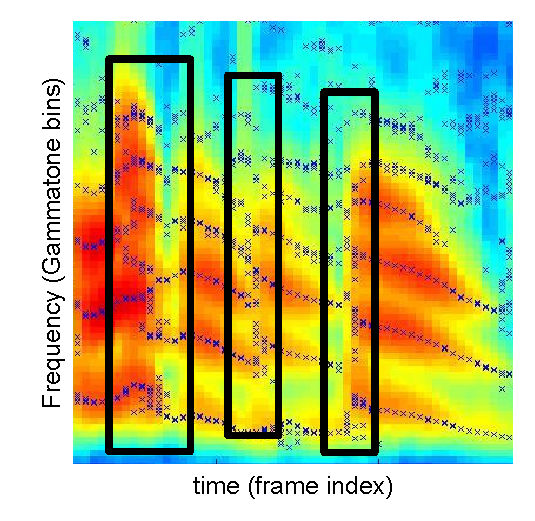
\includegraphics[height =2.0in, width=0.4\textwidth]{figures/co-channel_pyknogram-crop}
\vspace{-1mm}
\caption{A closer look on Pyknograms for overlapped speech. The enclosed patches show discontinuities that occur in the presence of an interfering speaker.}
\vspace{-1mm}
\label{fig:pyknograms_for_overlaps}
\end{figure}


We evaluate the performance of our proposed detection metric on overlapped speech from the GRID database~\cite{SSC_link}(see Sect.\ref{sec:exp} for more details on GRID). 
A key factor that determines the difficulty of detecting the presence of overlapped speech is the signal to interference(SIR) value. 
Greater absolute SIR values correspond to regions where one of the speakers has lower impact on the signal energy. 
Therefore it is more difficult to detect the occurrence of overlap in signals as the SIR moves away from $0dB$. 
Notice we use absolute SIR, since in overlap {\it detection} there is no difference between target and interfering speakers. 

Another important factor in detecting overlap is that the SIR value will change across different frames within a single file, which is due to the non-stationary nature of speech. 
This poses major restrictions on the effectiveness of overlap detection evaluation, since providing frame-based ground-truth becomes unrealistically difficult. 
One must therefore rely on ensemble measurements over complete speech files for which the average SIR is known. 
This notion is illustrated in Fig.~\ref{fig:compare_perframe_and_perfile_ovldethist}, where $D_{ovl}$ distributions (histograms) extracted on a per-frame basis are compared with ensemble $D_{ovl}$ distributions associated with each file. 
The ``scores'' ($D_{ovl}$ values) in Fig.~\ref{fig:compare_perframe_and_perfile_ovldethist} are pyknogram distances calculated using (\ref{eq:ovl_det_score}). 
The top figure (Fig.~\ref{fig:compare_perframe_and_perfile_ovldethist}-a), shows the distribution of scores per {\it frame} (i.e. $25$msec intervals) for overlapped (target) and clean (non-target/single-speaker) {\it files}.  
Figure~\ref{fig:compare_perframe_and_perfile_ovldethist}-b shows the ensemble score distributions (average score over all frames in a file, which are typically $2$ seconds long). 
The task in overlap detection is to separate the two classes in each plot (dark blue from light blue). 
As observed in these distributions, the per-frame classes are almost indistinguishable (Fig.~\ref{fig:compare_perframe_and_perfile_ovldethist}-a), while in Fig.~\ref{fig:compare_perframe_and_perfile_ovldethist}-b the classes show much better separation. 


\begin{figure}[h!]
	\centering
	\vspace{0mm}
    \textbf{Ensemble vs. frame-based decisioning}\par\medskip	
	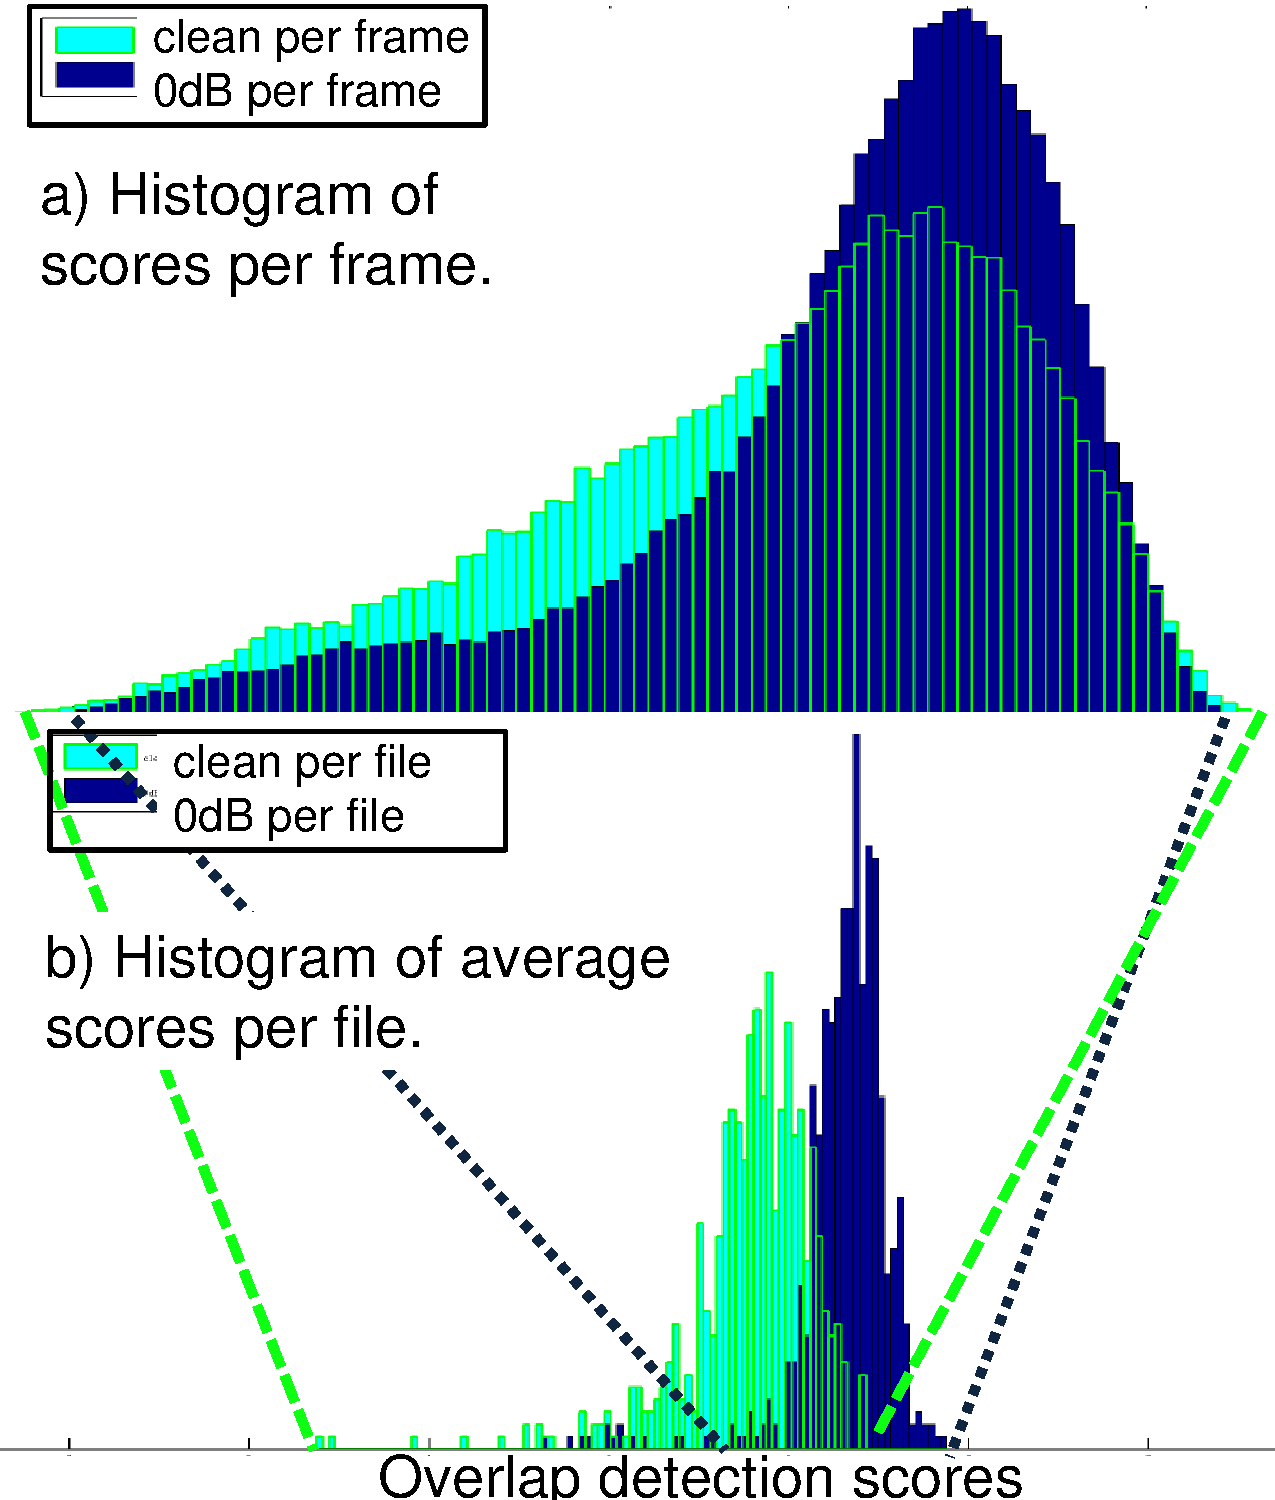
\includegraphics[height = 4in, width=0.5\textwidth]{figures/compare_pframe_pfile_hists}
	\vspace{-1mm}
	\caption{The effect of ensemble decisioning on distinguishability of overlapped regions. a) shows score per frame histograms and b) shows the histogram of ensemble scores. Using multiple frames to make a decision helps separate the distributions of clean and overlapped segments.}
	\vspace{-2mm}
	\label{fig:compare_perframe_and_perfile_ovldethist}
\end{figure}


%\subsection{HMM-based harmonic tracking for overlap detection}
%A more elaborate setup to track harmonic trajectories involves using a hidden Markov model (HMM) to model Pyknogram patterns. This allows for a supervised classification of speech segments into overlap and single-speaker speech. To do so, we propose using an initial segmentation of a given audio stream based on the Bayesian Information Criterion (BIC segmentation)~\cite{BIC}. The shorter segments are then compared against two pre-trained HMMs, one for overlapped and the other for single-speaker speech. The initial BIC segmentation is to allow for detection on shorter segments, since overlapped speech is considerably less frequent in a conversation compared to the total amount of speech. The combination of BIC segmentation and HMM-based classification allows for a practical overlap detection mechanism that fits well with analyzing conversations recorded in real conditions (as opposed to artificial datasets with simulated overlaps). Among other benefits of this framework is its compatibility with speaker diarization tools in which overlapped speech is considered a nuisance (see Sect.~\ref{sec:intro}). 

\newpage

\subsection{Evaluation}
\label{sec:exp}

This section evaluates our proposed pyknogram-based overlap detection system in terms of {\it accuracy, robustness,} and {\it precision}. 
Evaluation tasks for each SIR category are in the form of standard binary classification problems, where target examples are from a collection of files with fixed SIR values and non-target files are clean (single-speaker) files. 
We measure system performance using detection equal error-rates (EER; where false-positive and false-negative errors are equal). 
EER values are presented in Fig.~\ref{fig:ovl_det} for different SIRs. 
The expectation is that the detection algorithm should be consistent across a range of SIR values (i.e. robustness). 
As for precision, we are interested to know how short signals can be before overlap detection performance significantly drops (noting the observation in Fig.~\ref{fig:compare_perframe_and_perfile_ovldethist}). 


Bellow, a collection of overlap detection features are presented that have previously been used to detect overlapped regions~\cite{nav_icassp13,boakye_thesis,sapvr_2000}. 
%We note that all features were implemented based on the information provided in the publications, which are cited in each case. %adapted from other centers based on the information provided in publications. Although we tried to eliminate any chance of bias in the experiments, chances are that the results would have been different had the original authors implemented their methods for these experiments. 
To the best of our knowledge, overlap detection results on this database have not been reported for any of the following features, therefore we rely on our own implementations. %The out-of-house features used in this study are:


\subsubsection{Baseline features}

\label{ssec:baseline}
\begin{itemize}
  \item {\it Speech kurtosis}: Kurtosis has been reported as an effective measure to detect the presence of multiple speakers in overlapped signals by several studies~\cite{Wrigley_05,boakye_thesis,temple_kurtosis}. 
  It has been shown that overlapped speech exhibits lower kurtosis compared to single-speaker speech~\cite{leblanc_deleon98}. The kurtosis of a zero-mean random variable $x$ is defined as:

\begin{equation}
\label{eq:kurtosis}
k_x = \frac{E\{x^4\}}{(E\{x^2\})^2}
\end{equation}
\vspace{1mm}
In this case $x$ refers to speech samples in a given frame. 
  \item {\it Spectral flatness measure (SFM)}: The ratio of geometric to arithmetic means of spectral magnitudes across frequency within each frame~\cite{nav_icassp13}. For the $i^{th}$ frame:
\begin{equation}
\label{eq:kurtosis}
sfm_i = \frac{\frac{1}{N}\sum_{n=1}^{N}{X(f_n)}}{^N\sqrt{\prod_{n=1}^{N}{X(f_n)}}}
\end{equation}
\vspace{1mm}
where $X(f_n)$ corresponds to the magnitude spectrum at frequency $f_n$ and {N} is the total number of frequency bins. 
  \item {\it Spectral autocorrelation peak-valley ratio (SAPVR)}: described briefly in Sec.~\ref{sec:intro}, this feature uses the dominance of peaks in the spectral autocorrelation in each frame as a measure to detect overlaps~\cite{sapvr_2000}. 
\end{itemize}

\subsubsection{Data: Monaural Speech Separation Challenge}

The data used in our controlled experiments is from the monaural speech separation and recognition challenge (a.k.a speech separation challenge (SSC))~\cite{cooke20101}. 
The objective there was to permit a large-scale comparison of techniques for the overlapped speech problem~\cite{cooke20101}. 
Participants were asked to identify keywords in sentences spoken by a target talker when mixed into a single channel with a background talker speaking sentences of the same structure but with different content. 
The data used in SSC was obtained from the larger GRID corpus~\cite{cooke_JASA_SSCD}, which is a multi-talker audio-visual sentence corpus that supports computational-behavioral studies in speech perception. 
In our study, we only use the audio content which consists of 1000 sentences spoken by each of 34 talkers (18 male, 16 female). The sentences are structured in the following format.
\\\\
{\small \bf \textless command\textgreater\textless color\textgreater\textless preposition\textgreater\textless letter\textgreater\textless number\textgreater\textless code\textgreater}
\\\\
For example, ``lay white at X six now''.

The test and training set contain the same set of talkers. Seven overlapped sets are available, one clean and the rest composed of sentence pairs artificially summed at 6 signal-to-interference ratios (SIR) (+6, +3, 0, −3, −6, −9 dB). 
Since file durations are short (typically less than 5 seconds) and the utterances contain negligible pauses, it is reasonable to consider the average SIR values, provided for each file, a fair representation of the amount of overlap. 
This also allows the assumption that the entire signal is overlapped (see Fig.~\ref{fig:overlap_example}). 
We have down-sampled all files to 8kHz to match telephone recordings. 
Note that the experiments conducted in this study do not comply with the objectives of the speech separation challenge described in~\cite{SSC_link}. 

% Figure added because of Reviewer3 and 1's comment:
\vspace{0mm}
\begin{figure}[h!]
	\centering
	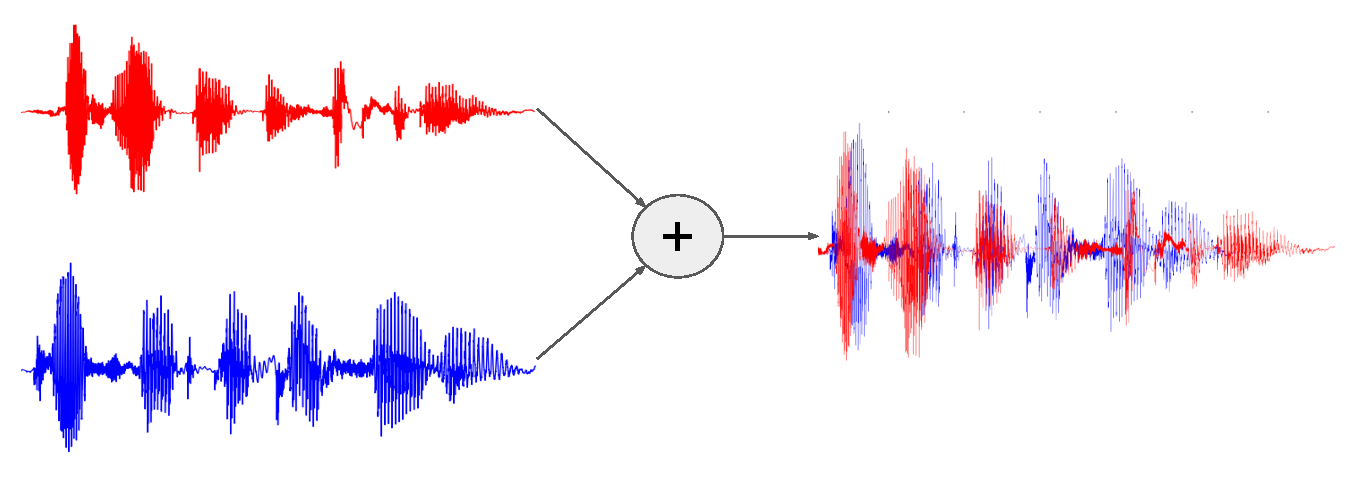
\includegraphics[height =1.8in, width=0.7\textwidth]{figures/GRID_example_overlap-crop}
	\vspace{-2mm}
	\caption{
		Example of the mixing process for a 0dB SIR overlapped signal. As shown on the right, it is fair to assume that overlap occurs throughout the signal.}
	\label{fig:overlap_example}
\end{figure}

% Reviewer1's comment:
This corpus is isolated from variabilities other than overlapped speech, which makes it useful to study the effects of overlap. 
To the best of our knowledge, this dataset is the most organized publicly available corpus that contains large, as well controlled, amounts of overlapped speech (note that we are mostly interested in {\it overlapped speech} and not {\it co-channel speech} as defined and distinguished in the introduction). 
Among the corpus' other advantages is the fact that segments are short which makes the definition of a signal-to-interference ratio more appropriate. Had the signals been longer, say a few minutes long, the notion of a signal-to-interference ratio across the entire signal would have been less applicable, due to the non-stationary nature of speech. 

\begin{table}[h!]
	\begin{center}
		\label{tab:data_summary}
		\begin{tabular}{| c | c |}
			\hline
			\hline
			number of speakers	& 18 (male)  \\
			\hspace{4mm}			&  16 (female) \\
			\hline
			average file duration	&   1.9 (sec) \\ 
			\hline
			noise				& interfering speakers \\
			\hspace{4mm}			& clean,$+6$, $+3$, $0$, $-3$, $-6$, $-9$ dB \\
			\hline
			sampling rate			& $8$ KHz \\
			\hline
			\hline	
		\end{tabular}
		\caption{Summary of data used for SID experiments}
	\end{center}
\end{table}


\vspace{3mm}
\subsubsection{Overlapped speech detection vs. SIR (Robustness \& Accuracy)}
Here the performance of pyknogram-based overlap detection is compared with the three baseline algorithms across different SIR values. 
The goal is to monitor the chances in EER as SIR values increase. 
The target/non-target files used in this binary classification task are obtained from a pool of overlapped and clean files. 
In each task, overlapped files with the same SIR are used as target examples and the overlap detection score (or feature value) assigned to them is compared against the scores estimated for clean files to compute the binary classification EER. 
Figure~\ref{fig:ovl_det} compares performances for the proposed and baseline systems across SIR values of $0, 3, 6$ and $9dB$.

\begin{figure}[h!]
	\centering
	\hspace{-1mm}
	\textbf{Overlap Detection vs. SIR}\par\medskip
	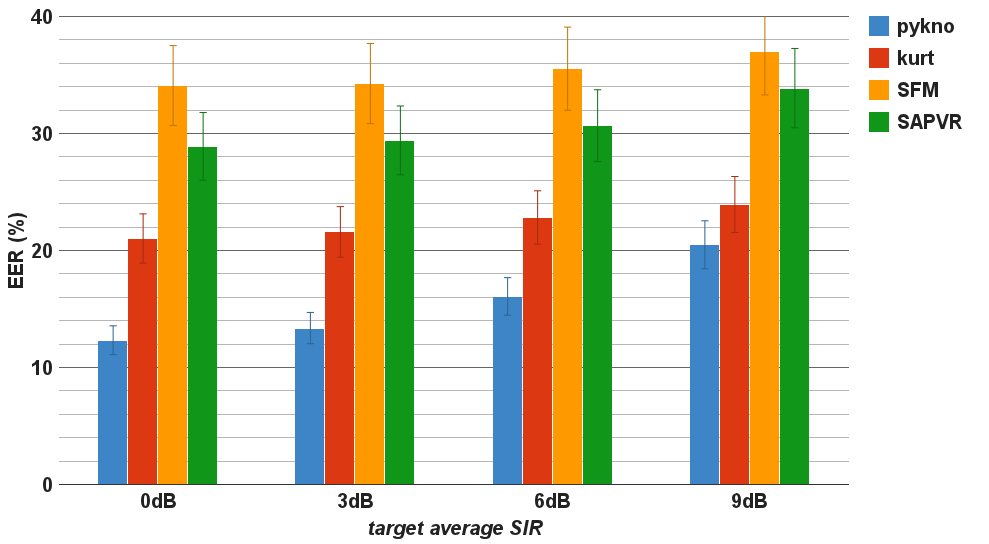
\includegraphics[height = 3.1in, width=0.7\textwidth]{figures/ovldet_vs_sir}
	\vspace{-1mm}
	\caption{Overlap detection EER for different SIR values. The higher the SIR, the more difficult it is to detect the presence of interfering speakers.}
	\vspace{0mm}
	\label{fig:ovl_det}
\end{figure}



\newpage
\subsubsection{Overlapped speech detection vs. segment length}
A main concern in dealing with overlapped regions is that overlap decisions are less reliable as segment lengths become shorter. 
This restricts algorithm precision in terms of the ability to detect overlap in a frame-based framework. 
Precision is most valuable in tasks such as speaker diarization in conversational speech, where overlap mostly occurs at speaker transitions in turn-takings. 
The goal of this phase is to evaluate system precision and compare pyknogram-based detection with baseline features. 
In other words, how short can overlap segments get before observing a significant drop in system performance. 
Once again, overlap detection performance is measured through the detection EER. 
Figure~\ref{fig:ovl_det_precision} shows the change in system performance as shorter duration segments are used to obtain overlap decisions. 


\begin{figure}[h!]
	\centering
	\hspace{-1mm}
	\textbf{Precision of Overlap Detection methods}\par\medskip
	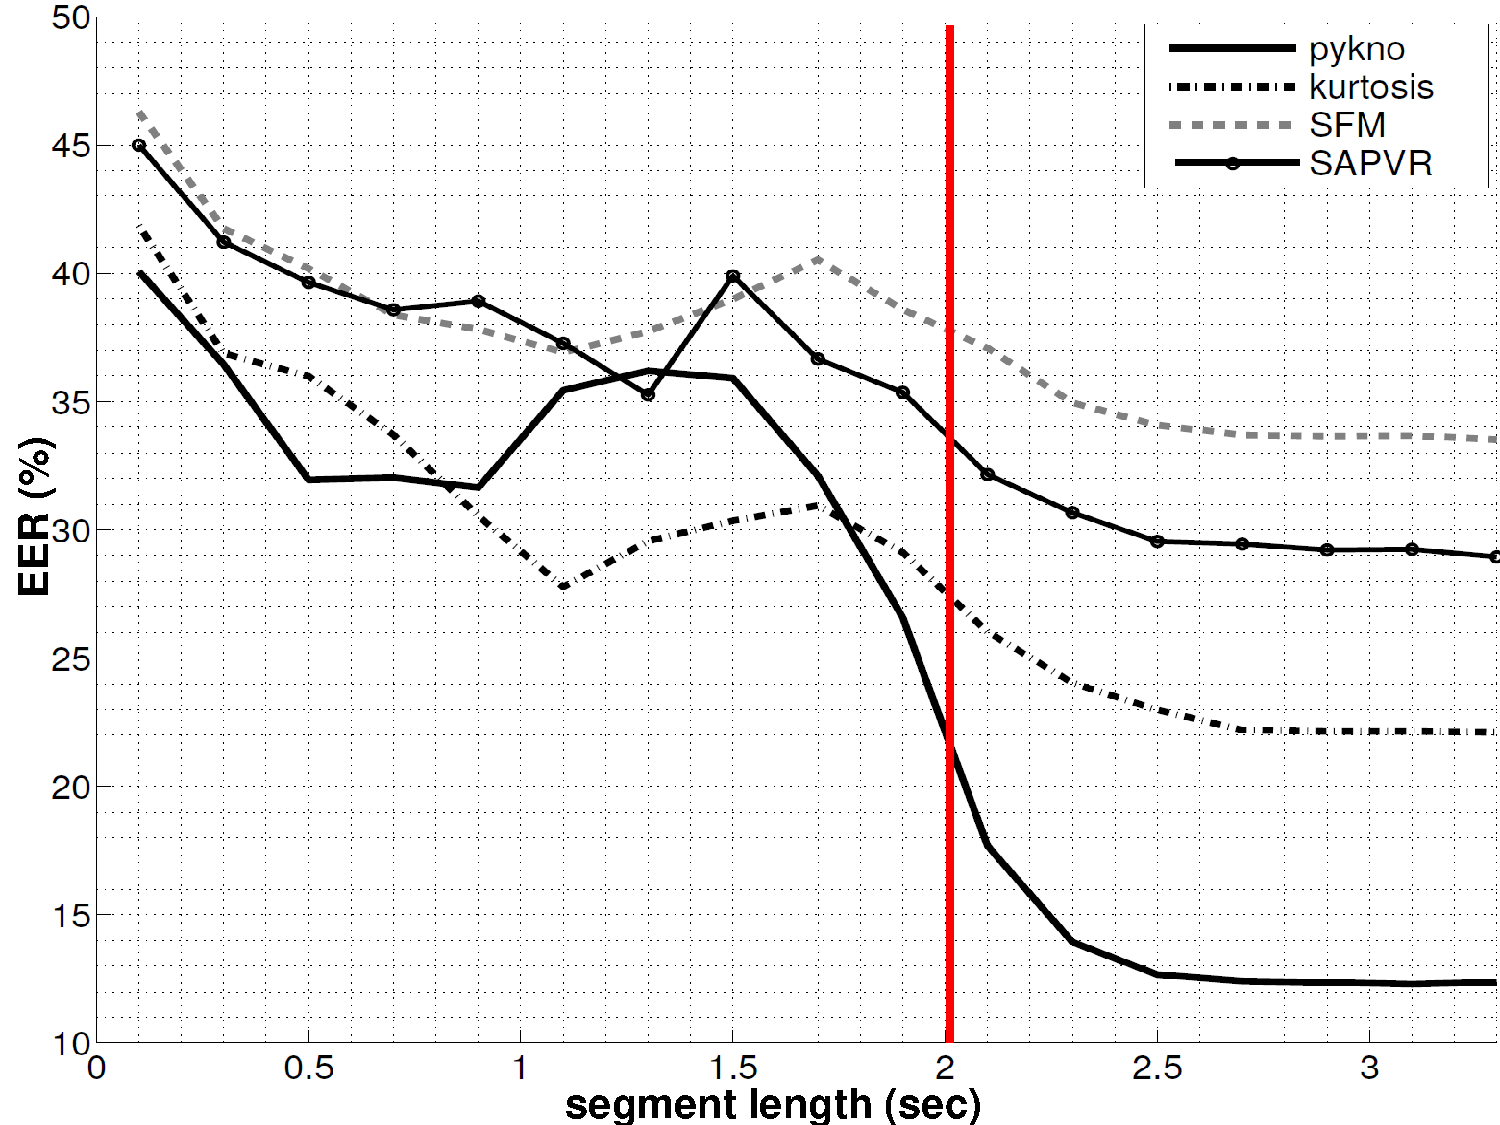
\includegraphics[height = 3.1in, width=0.5\textwidth]{figures/eer_vs_time}
	\vspace{-1mm}
	\caption{Overlap detection EER as a function of segment length. The plot shows that signal lengths should be at least $2$ seconds for the algorithms to start reaching their best performance.}
	\vspace{0mm}
	\label{fig:ovl_det_precision}
\end{figure}


\section{Gammatone Sub-band Frequency Modulation Spectra}
\label{sec:GSFM}

